\documentclass[11pt,letter]{article}
\usepackage{etex}
\usepackage[top=0.65in,bottom=0.9in,left=0.85in,right=0.85in]{geometry}

%\def\baselinestretch{1.25}
\def\baselinestretch{1.0}

\usepackage[greek, english]{babel}
%\usepackage{multicol}
\usepackage[thinlines]{easytable}

%\usepackage[draft]{graphicx}
\usepackage{graphicx}
\usepackage[export]{adjustbox}

\usepackage{caption}
\usepackage{subcaption}

\usepackage{setspace}
\usepackage{float}

% The use of the times package forces the use of the type-1 times
% roman font, but the times roman font does not look nice.
% Besides the times roman font still does not print correctly on
% the dopy printer.
%\usepackage{times}


\usepackage{fancyhdr}
\usepackage{amsmath}
\usepackage{amssymb}
\usepackage{bm}
\usepackage{bbold}
\usepackage{parskip}
\usepackage{url}

\newcommand{\kb}{\ensuremath{k_{\text{B}}}}

\newcommand{\bv}[1]{\ensuremath{\bm{#1}}}
\newcommand{\Lc}{\ensuremath{L_{\mathrm{c}}}}
\newcommand{\dsig}[1]{\ensuremath{ \frac{ d\,\sigma_{#1} }{d\,\Omega} }}

\newcommand{\isat}{\ensuremath{I_{\mathrm{sat}}}}
\newcommand{\iisat}{\ensuremath{I_{\mathrm{p}}/I_{\mathrm{sat}}}}
\newcommand{\Iqtof}{\ensuremath{I_{\bv{Q}\infty} }}
\newcommand{\Itof}[1]{\ensuremath{I_{\bv{#1}\infty} }}
\newcommand{\Iq}{\ensuremath{I_{\bv{Q}} }}
\newcommand{\iq}{\ensuremath{i_{\bv{Q}} }}
\newcommand{\Iqma}{\ensuremath{I_{\bv{Q}_{\text{MA}}} }}
\newcommand{\Ima}[1]{\ensuremath{I_{\bv{#1}_{\text{MA}}} }}
\newcommand{\iqma}{\ensuremath{i_{\bv{Q}_{\text{MA}}} }}
\newcommand{\jqma}{\ensuremath{j_{\bv{Q}_{\text{MA}}} }}
\newcommand{\Iqmatof}{\ensuremath{I_{\bv{Q}_{\text{MA}\infty}} }}
\newcommand{\is}{\ensuremath{i_{S}} }
\newcommand{\iqT}{\ensuremath{i_{\bv{Q}_{T}} }}
\newcommand{\ipith}{\ensuremath{i_{\bv{\pi}/\bv{\theta}}}}
\newcommand{\fpith}{\ensuremath{f_{\bv{\pi}/\bv{\theta}}}}
\newcommand{\iT}[1]{\ensuremath{i_{\bv{#1}_{T}} }}
\newcommand{\ima}[1]{\ensuremath{i_{\bv{#1}_{\text{MA}}} }}
\newcommand{\fma}[1]{\ensuremath{f_{\bv{#1}_{\text{MA}}} }}
\newcommand{\jma}[1]{\ensuremath{j_{\bv{#1}_{\text{MA}}} }}

\newcommand{\pin}{\ensuremath{ P_{\text{i}}} }
\newcommand{\pret}{\ensuremath{ P_{\text{r}}} }
\newcommand{\win}{\ensuremath{ w_{\text{in}}} }
\newcommand{\wret}{\ensuremath{ w_{\text{r}}} }
\newcommand{\wir}{\ensuremath{ w_{\text{IRS}}} }

\newcommand{\pgr}{\ensuremath{ P_{\text{gr}}} }
\newcommand{\wgr}{\ensuremath{ w_{\text{gr}}} }

\newcommand{\dbl}{\ensuremath{ \!\uparrow\! \downarrow \, }}
\newcommand{\spup}{\ensuremath{ \!\uparrow }}
\newcommand{\spdn}{\ensuremath{ \!\downarrow}}

\newcommand{\rdiag}{\ensuremath{ r_{\text{\tiny{111}}} } }
\newcommand{\awaist}{\ensuremath{ \alpha_{w} }}  
\newcommand{\awaistevap}{\ensuremath{ \alpha_{w,\text{evap}} }}  

\begin{document}

\section{LDA results as a function of atom number} 

In the previous update we showed LDA results in which the trap geometry and
temperature $T$ were kept constant and the atom number was varied.  We have
now pushed the accessible temperatures down a little bit which allows the LDA
to match our experimental data.  

We show again, in Figs.~\ref{fig:200a0_varyN}-\ref{fig:470a0_varyN}, some
results as a function of atom number for the coldest $T$ accessible at each
of the four values of the interaction strength relevant for comparison with
the experiment. 

This time we have included additional plots in the results graphic.  The
additional quantities that we are showing  are:

\begin{centering}
\begin{tabular}{c|p{11cm}}
 $n$& density exclusively from QMC data (circles) is shown alongside
the density from NLCE data (lines) \\[0.6em] $s$ & entropy per lattice
site at radius $r_{111}$ \\[0.6em] $4\pi r^{2} n $ & Number of atoms in shell
at $r_{111}$ (per shell thickness) \\[0.6em] $4\pi r^{2} S_{\pi} $ &
Structure factor in shell at $r_{111}$ (per shell thickness) \\[0.6em] $4\pi
r^{2} s $ &   Entropy per lattice site in shell at $r_{111}$ (per shell
thickness) \\[0.6em] $s/n$ & entropy per particle at radius $r_{111}$
\\[0.6em]
\end{tabular} 
\end{centering}

Keep in mind that we have trouble accessing QMC data for large radii, at the
edge of the cloud,  where the local value of $T/t$ is very low.   For this
reason we are forced to cutoff the LDA at a certain radius.  The cutoff
radius is the same for the various quantities, i.e. $S_{\pi}/n$, $s$, and $n$
(For $n$ the cutoff is only relevant for the value of $n$ obtained from QMC
data (circles)).   It can be seen that for $S_{\pi}/n$ the cutoff radius does
not pose a problem,  we see $S_{\pi}/n$ go smoothly to 1 at large radii.  On
the other hand the entropy per lattice site suffers an abrupt cutoff.  

At the moment we care the most about  $\bar{S}_{\pi}$ so we will ignore the
cutoff issue in $s$.  More QMC data will be required to solve this problem.

\begin{figure}[H]
    \centering
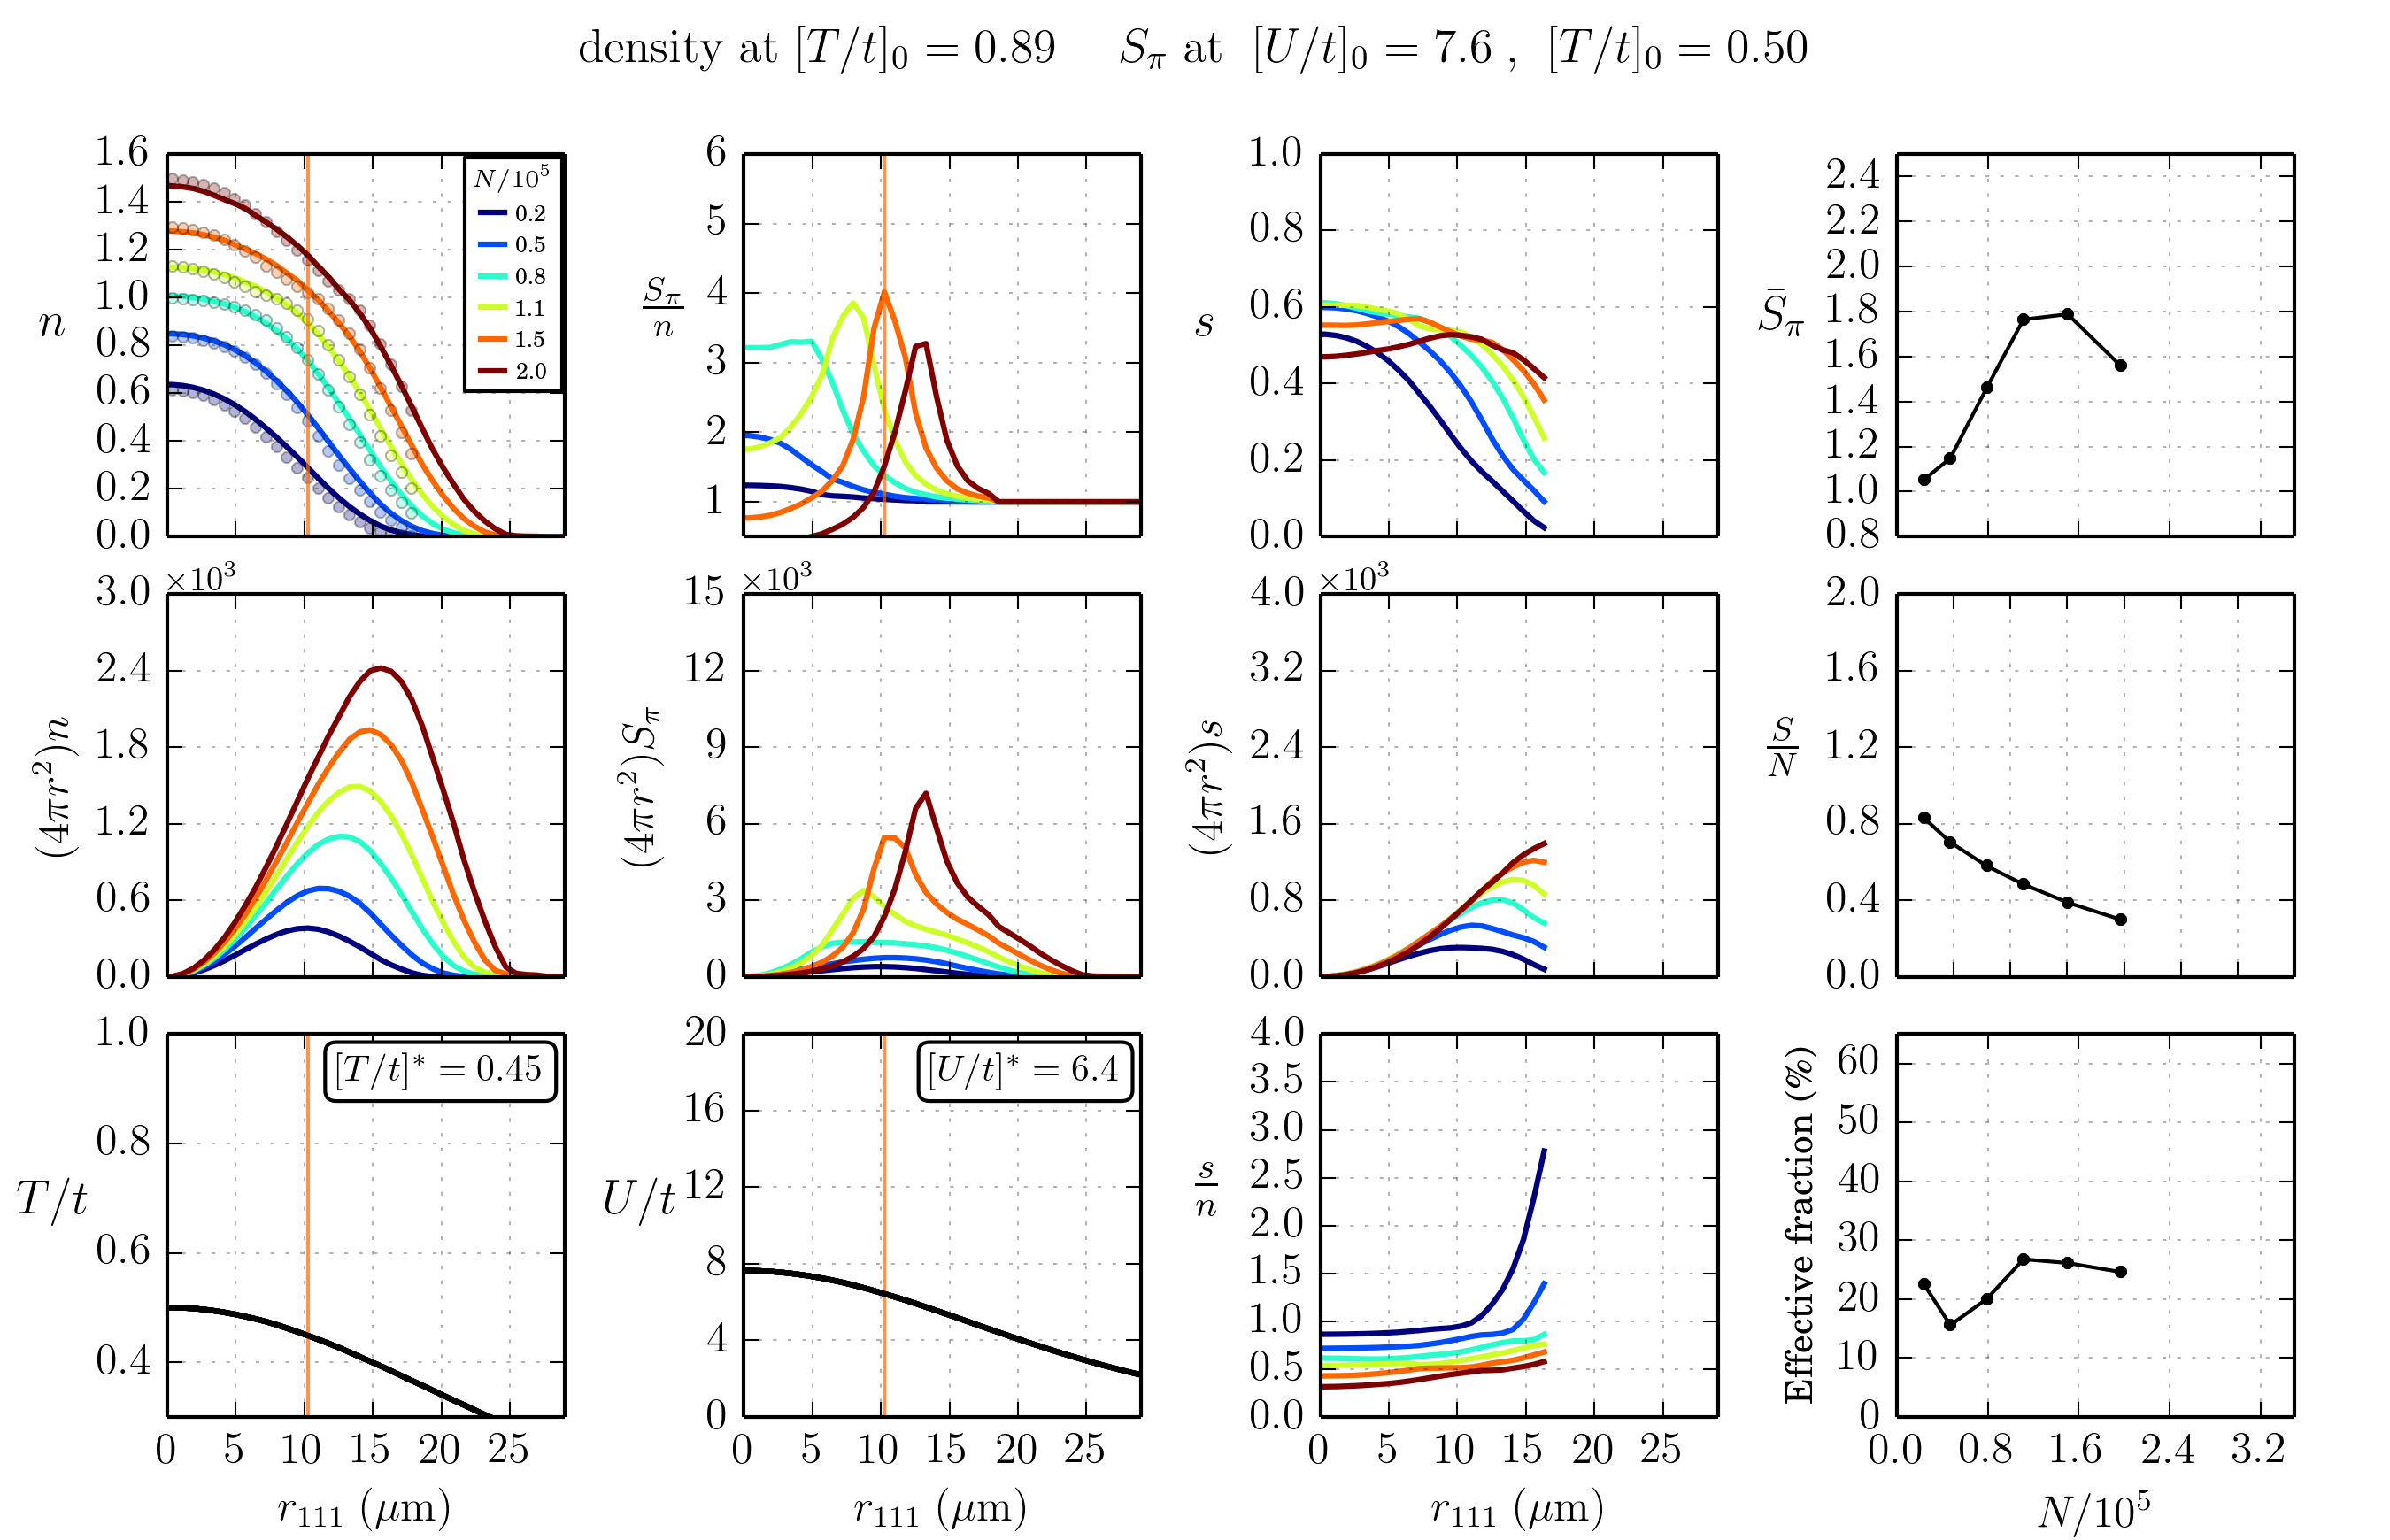
\includegraphics[width=0.95\textwidth]{figures/200a0_cold.png}
\caption{Scattering length 200\,$a_{0}$ ($[U/t]_{0}=7.6$).  Variation of
various quantities with atom number. } 
\label{fig:200a0_varyN}
\end{figure}
\begin{figure}[H]
    \centering
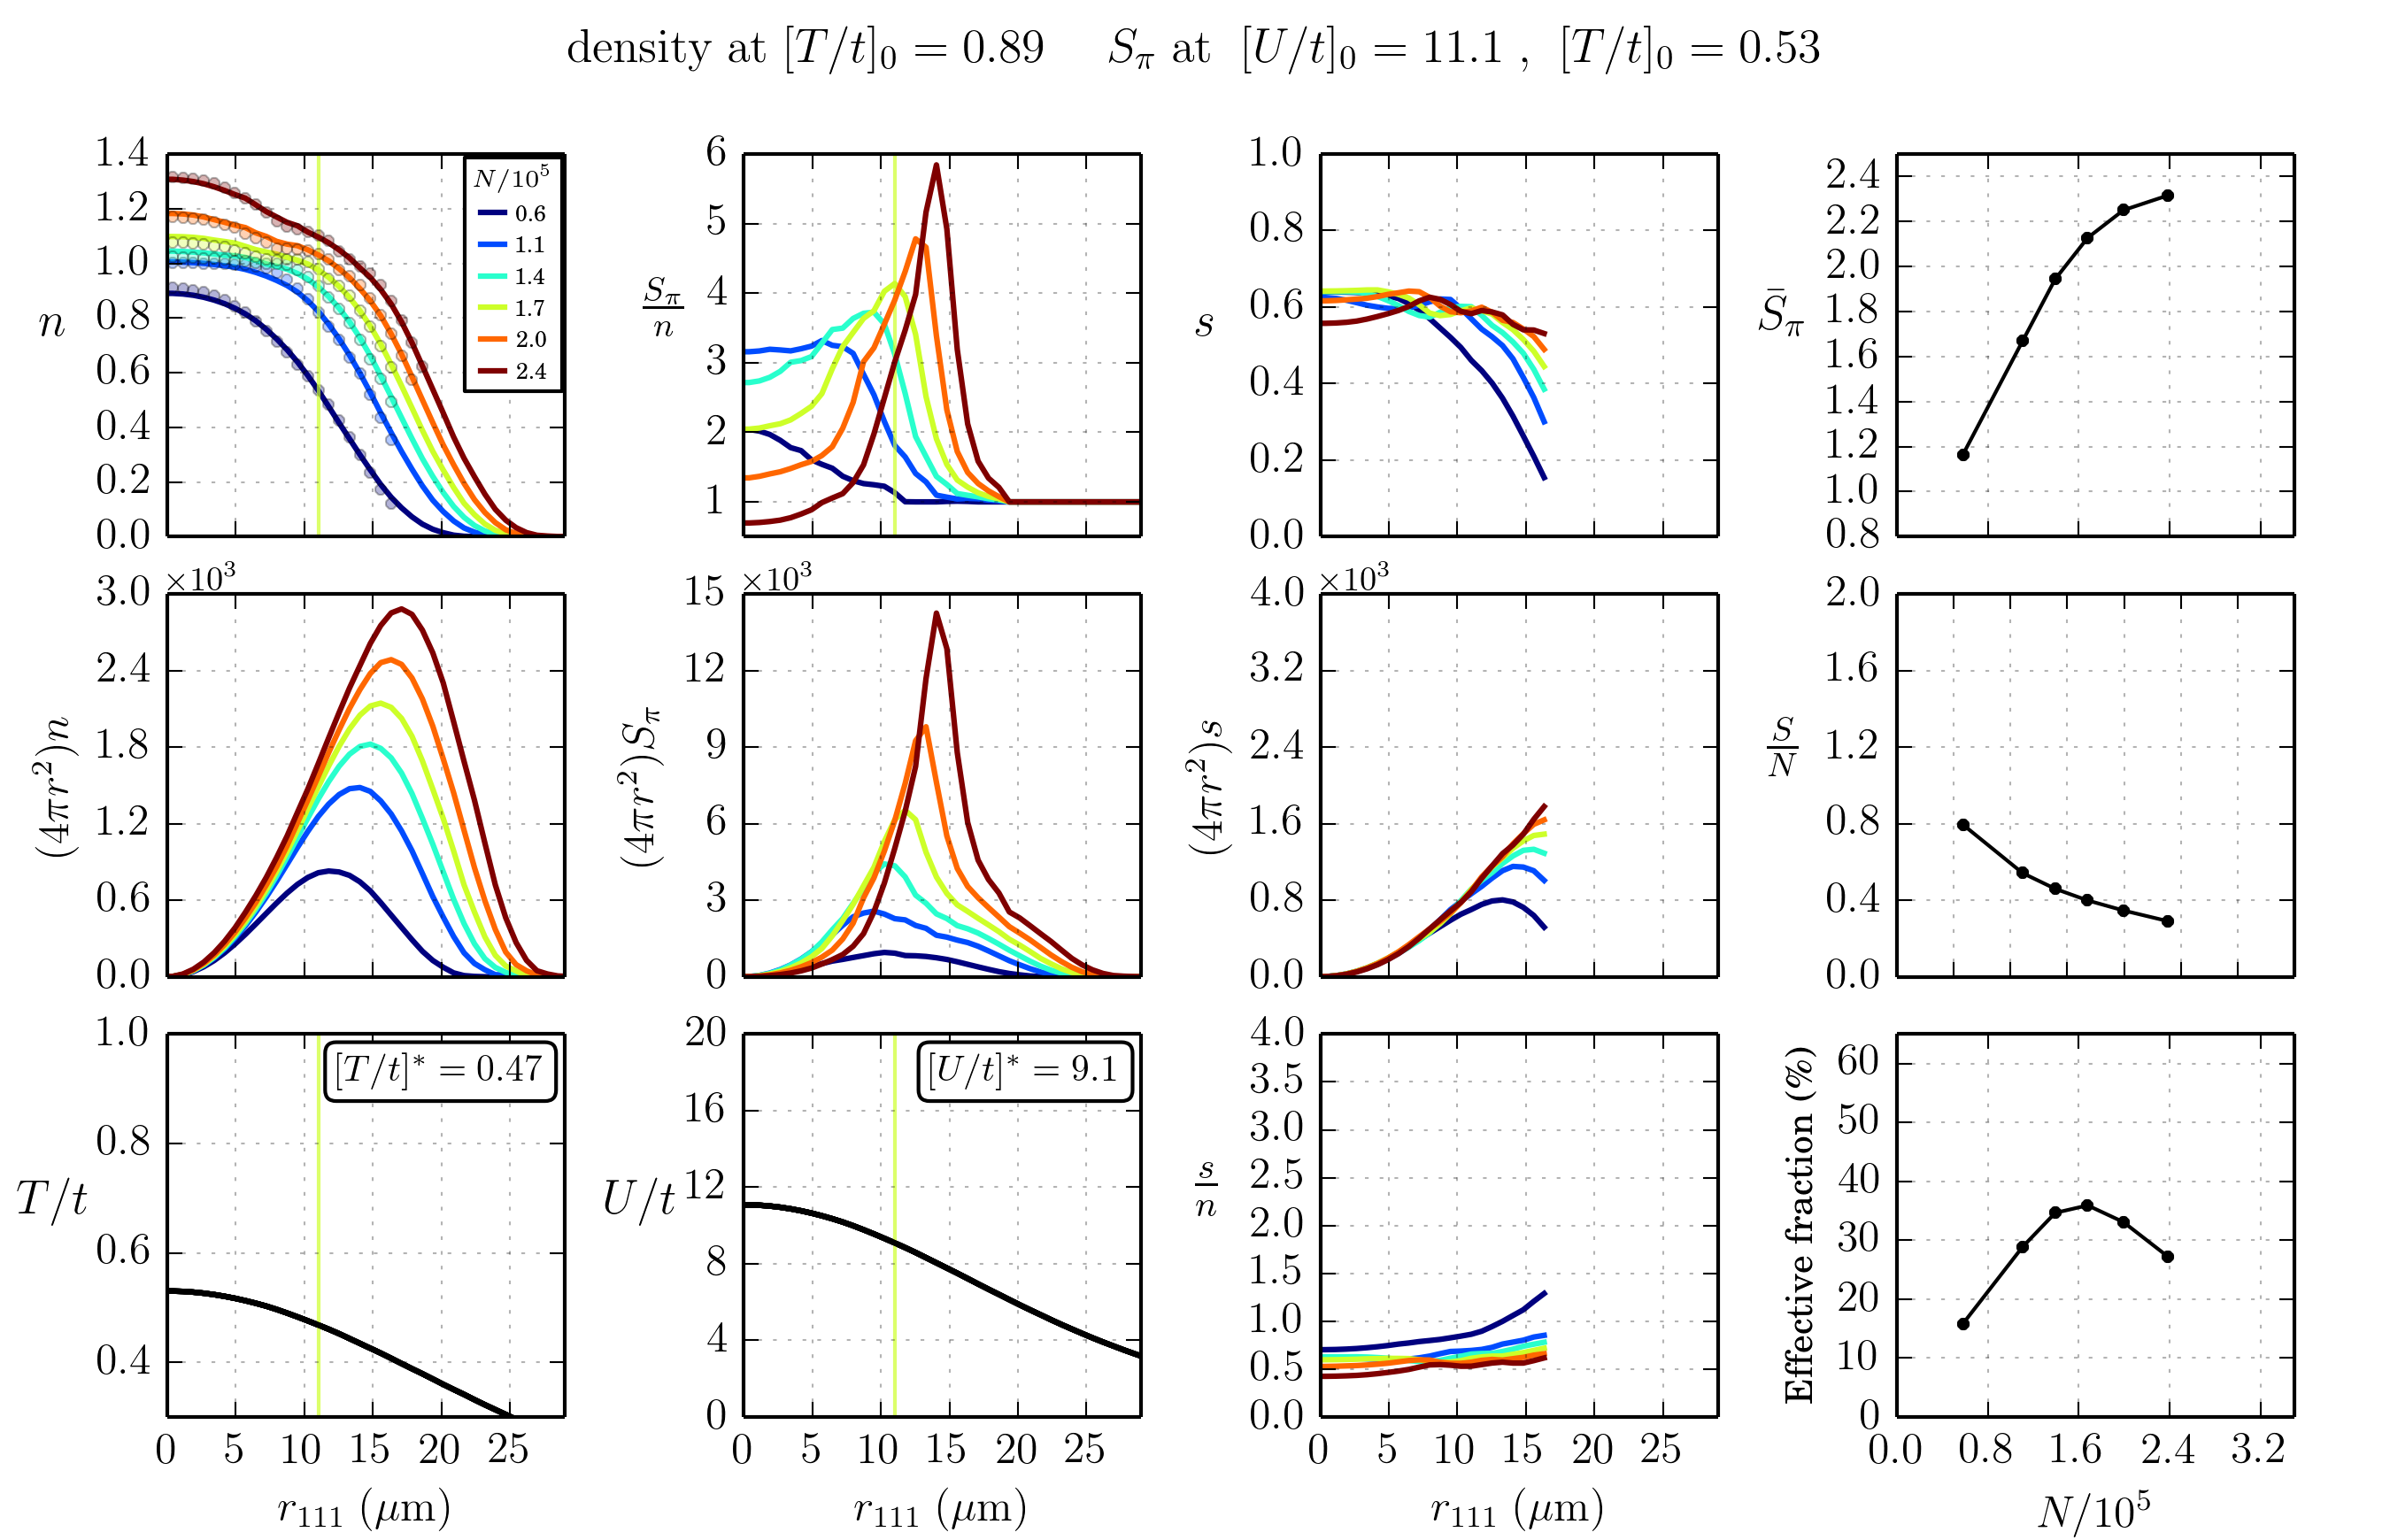
\includegraphics[width=0.95\textwidth]{figures/290a0_cold.png}
\caption{Scattering length 290\,$a_{0}$ ($[U/t]_{0}=11.1$).   } 
\label{fig:290a0_varyN}
\end{figure}
\begin{figure}[H]
    \centering
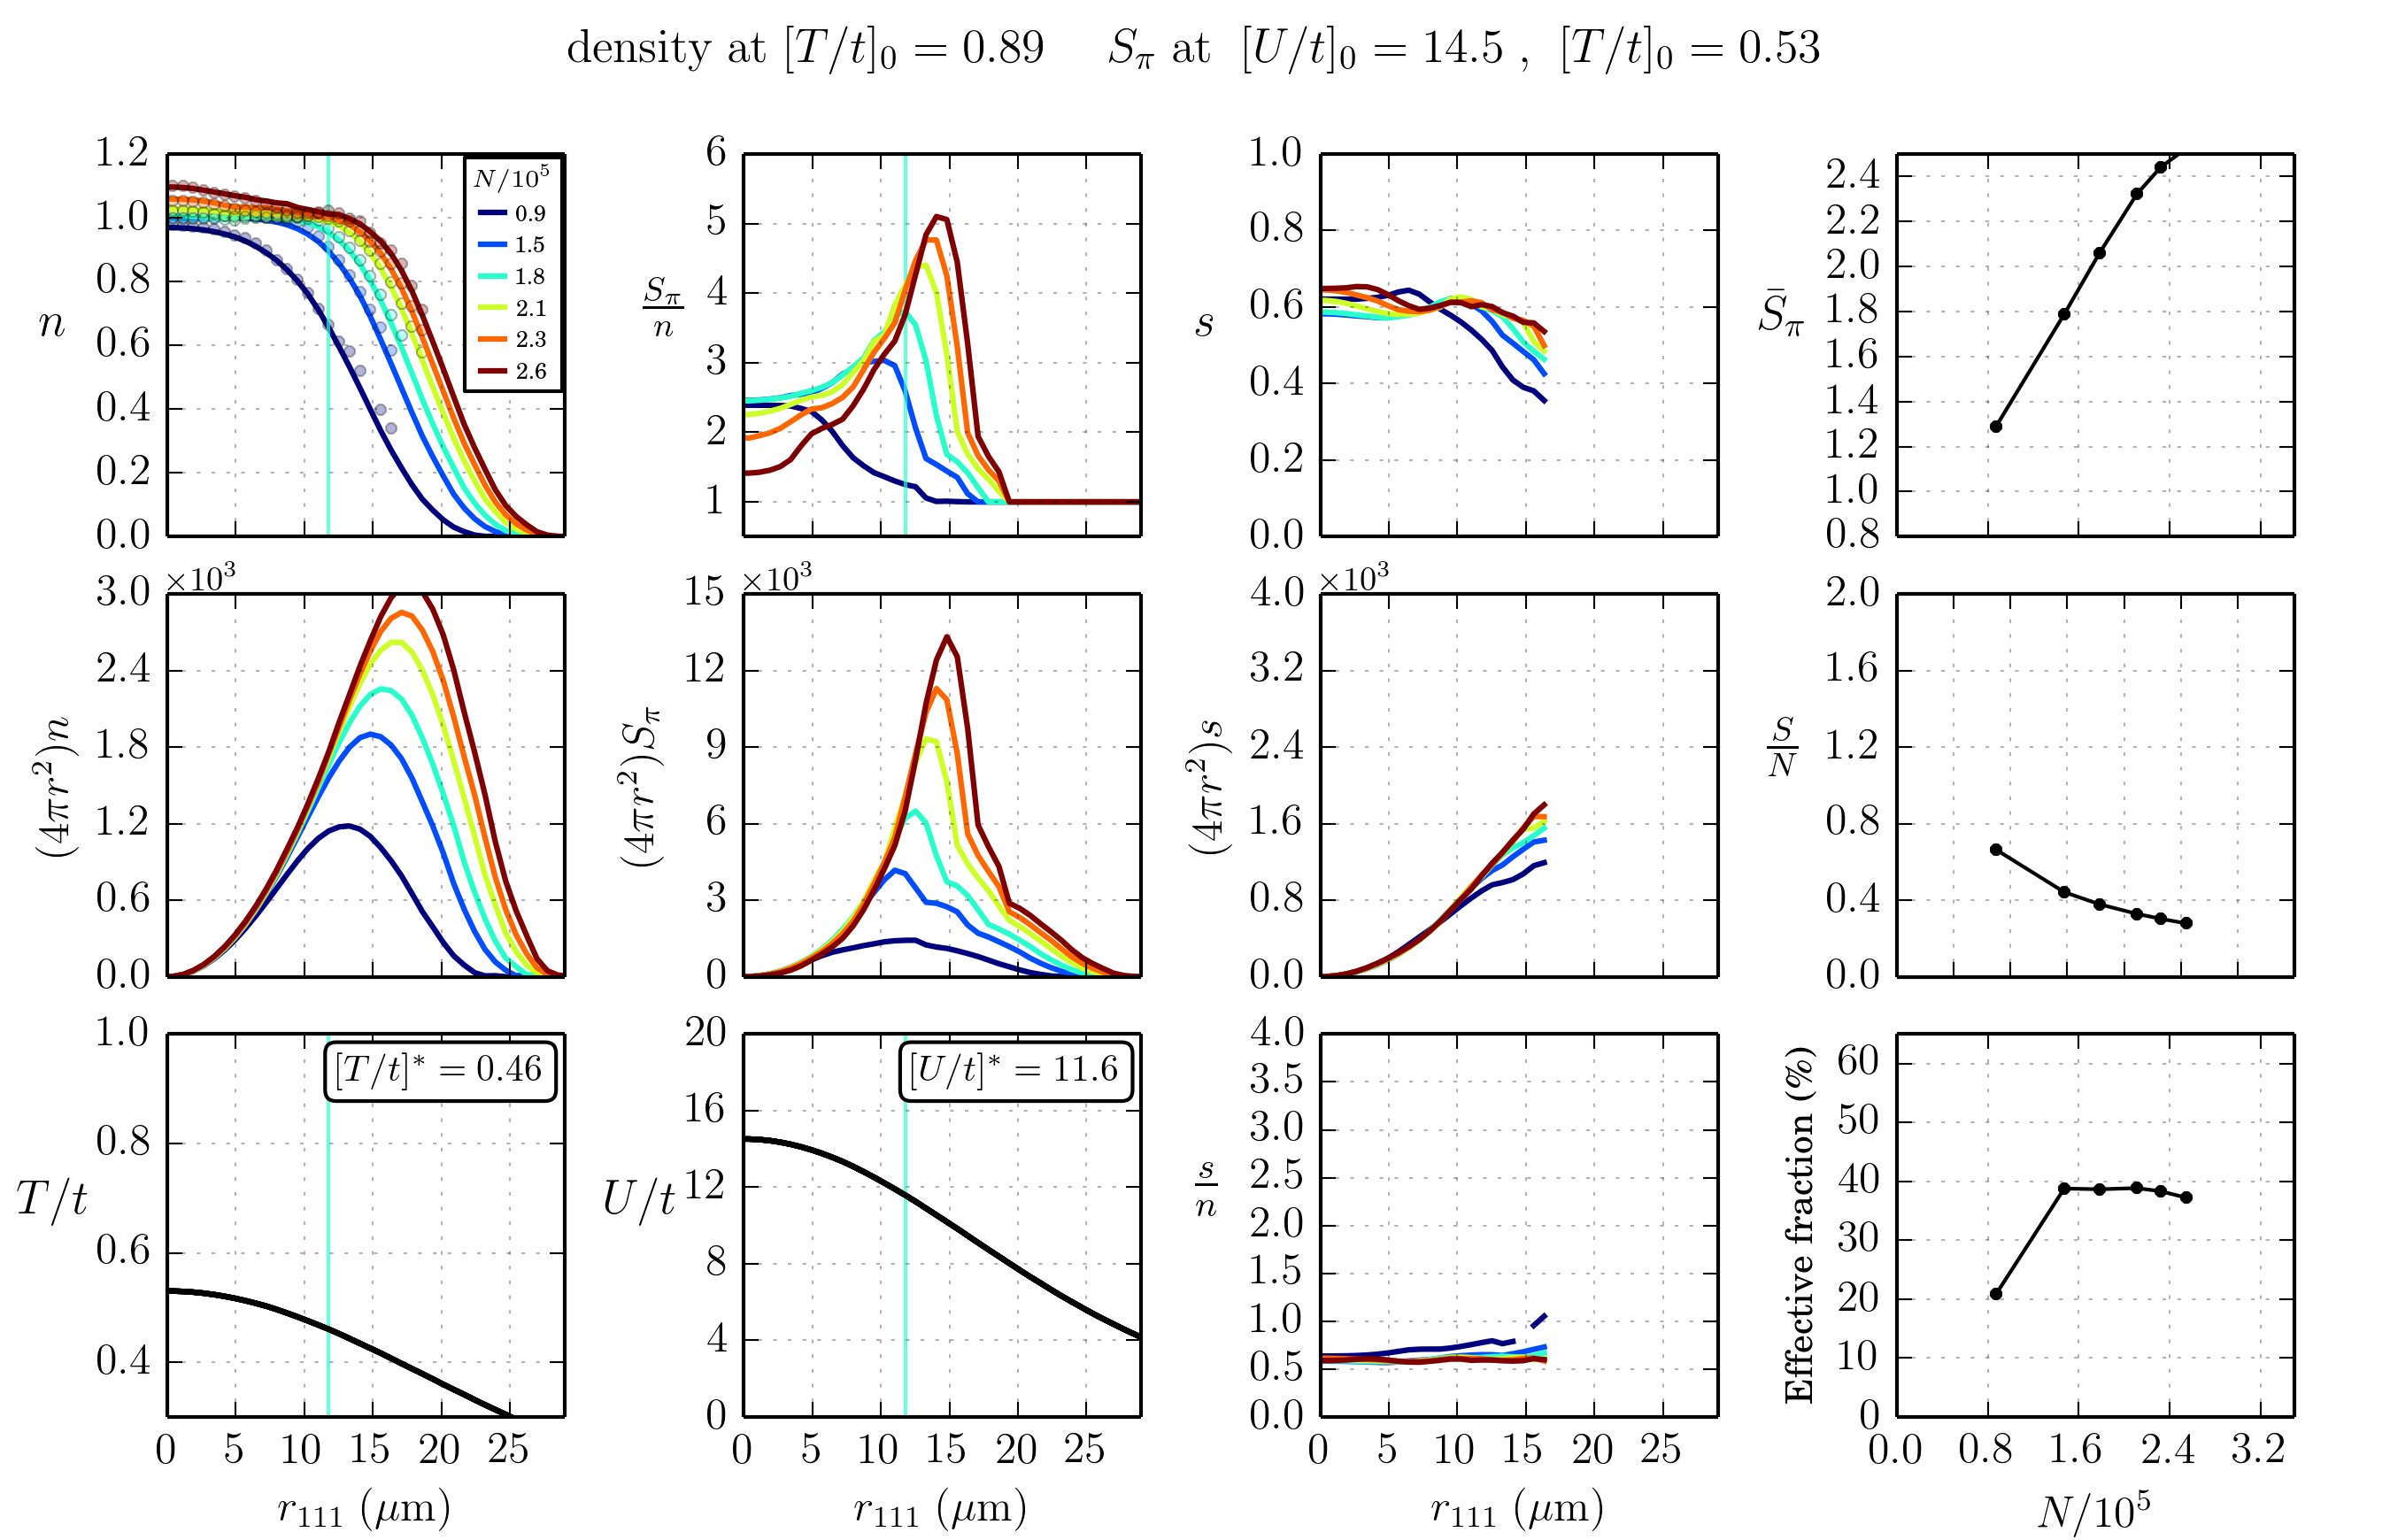
\includegraphics[width=0.95\textwidth]{figures/380a0_cold.png}
\caption{Scattering length 380\,$a_{0}$ ($[U/t]_{0}=14.5$).   } 
\label{fig:380a0_varyN}
\end{figure}
\begin{figure}[H]
    \centering
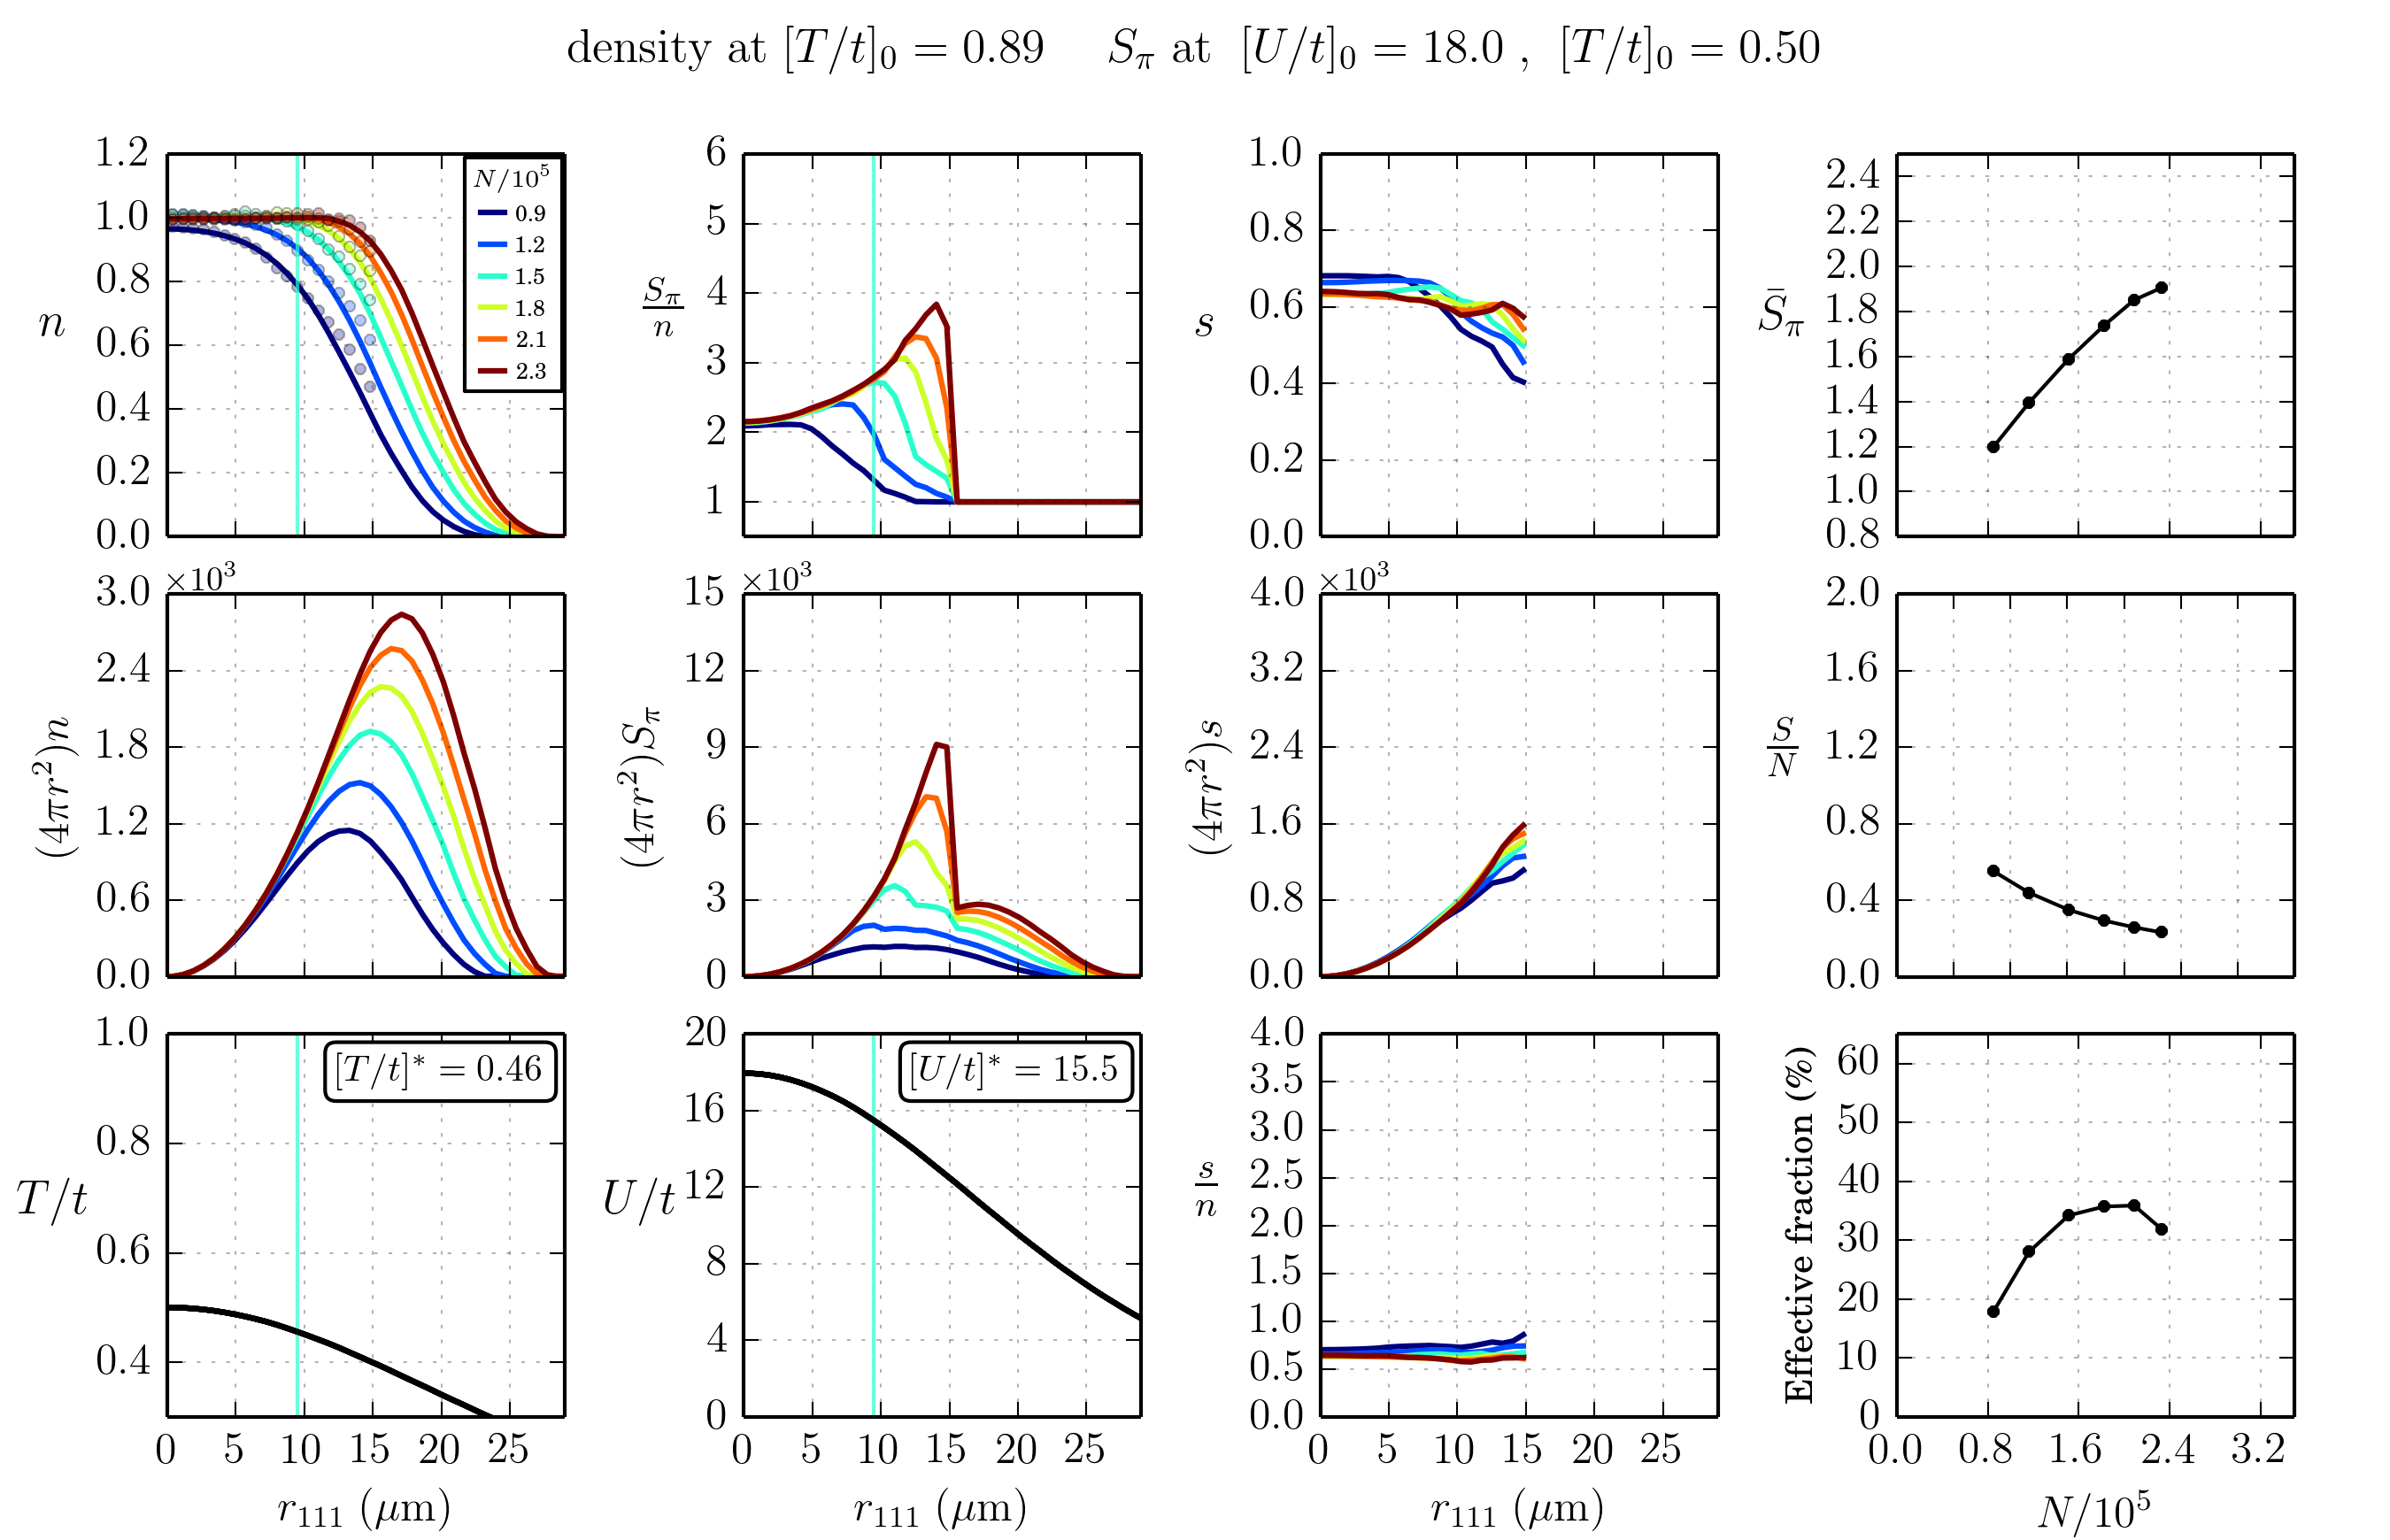
\includegraphics[width=0.95\textwidth]{figures/470a0_cold.png}
\caption{Scattering length 470\,$a_{0}$ ($[U/t]_{0}=18.0$).   } 
\label{fig:470a0_varyN}
\end{figure}
 


\section{Entropy capacity of the wings} 

After the last report, Nandini suggested that we looked at the entropy
profiles to assess the degree of entropy redistribution going on at the wings
of the sample.   For the LDA at the lowest $T$ we cannot access the local
entropy at the wings;  so, in
Figs.~\ref{fig:200a0_varyNhot}-\ref{fig:470a0_varyNhot} we show results for a
a slightly larger temperature, $[T/t]_{0}=0.68$.   In that case we can sample
larger radii with the QMC data and we observe the expected entropy
redistribution by noticing that $s/n$ grows quickly at large radii.
 
\section{Comment on overall entropy per particle $S/N$}

Looking at Figs.~\ref{fig:200a0_varyNhot}-\ref{fig:470a0_varyNhot}, in the
panel that shows $S/N$ vs $N$ we can see that, when the atom number is varied
at constant $T$, the overall entropy per particle $S/N$ decreases for larger
atom number.  

The plot that shows $\bar{S}_{\pi}$ vs. $N$ is a constant $T$ plot, but for a
better comparison with the experiment it should rather be a constant $S/N$
plot.  At the low temperatures we cannot calculate $S/N$ properly because we
do not have all of the necessary entropy data from QMC.   

\begin{figure}[H]
    \centering
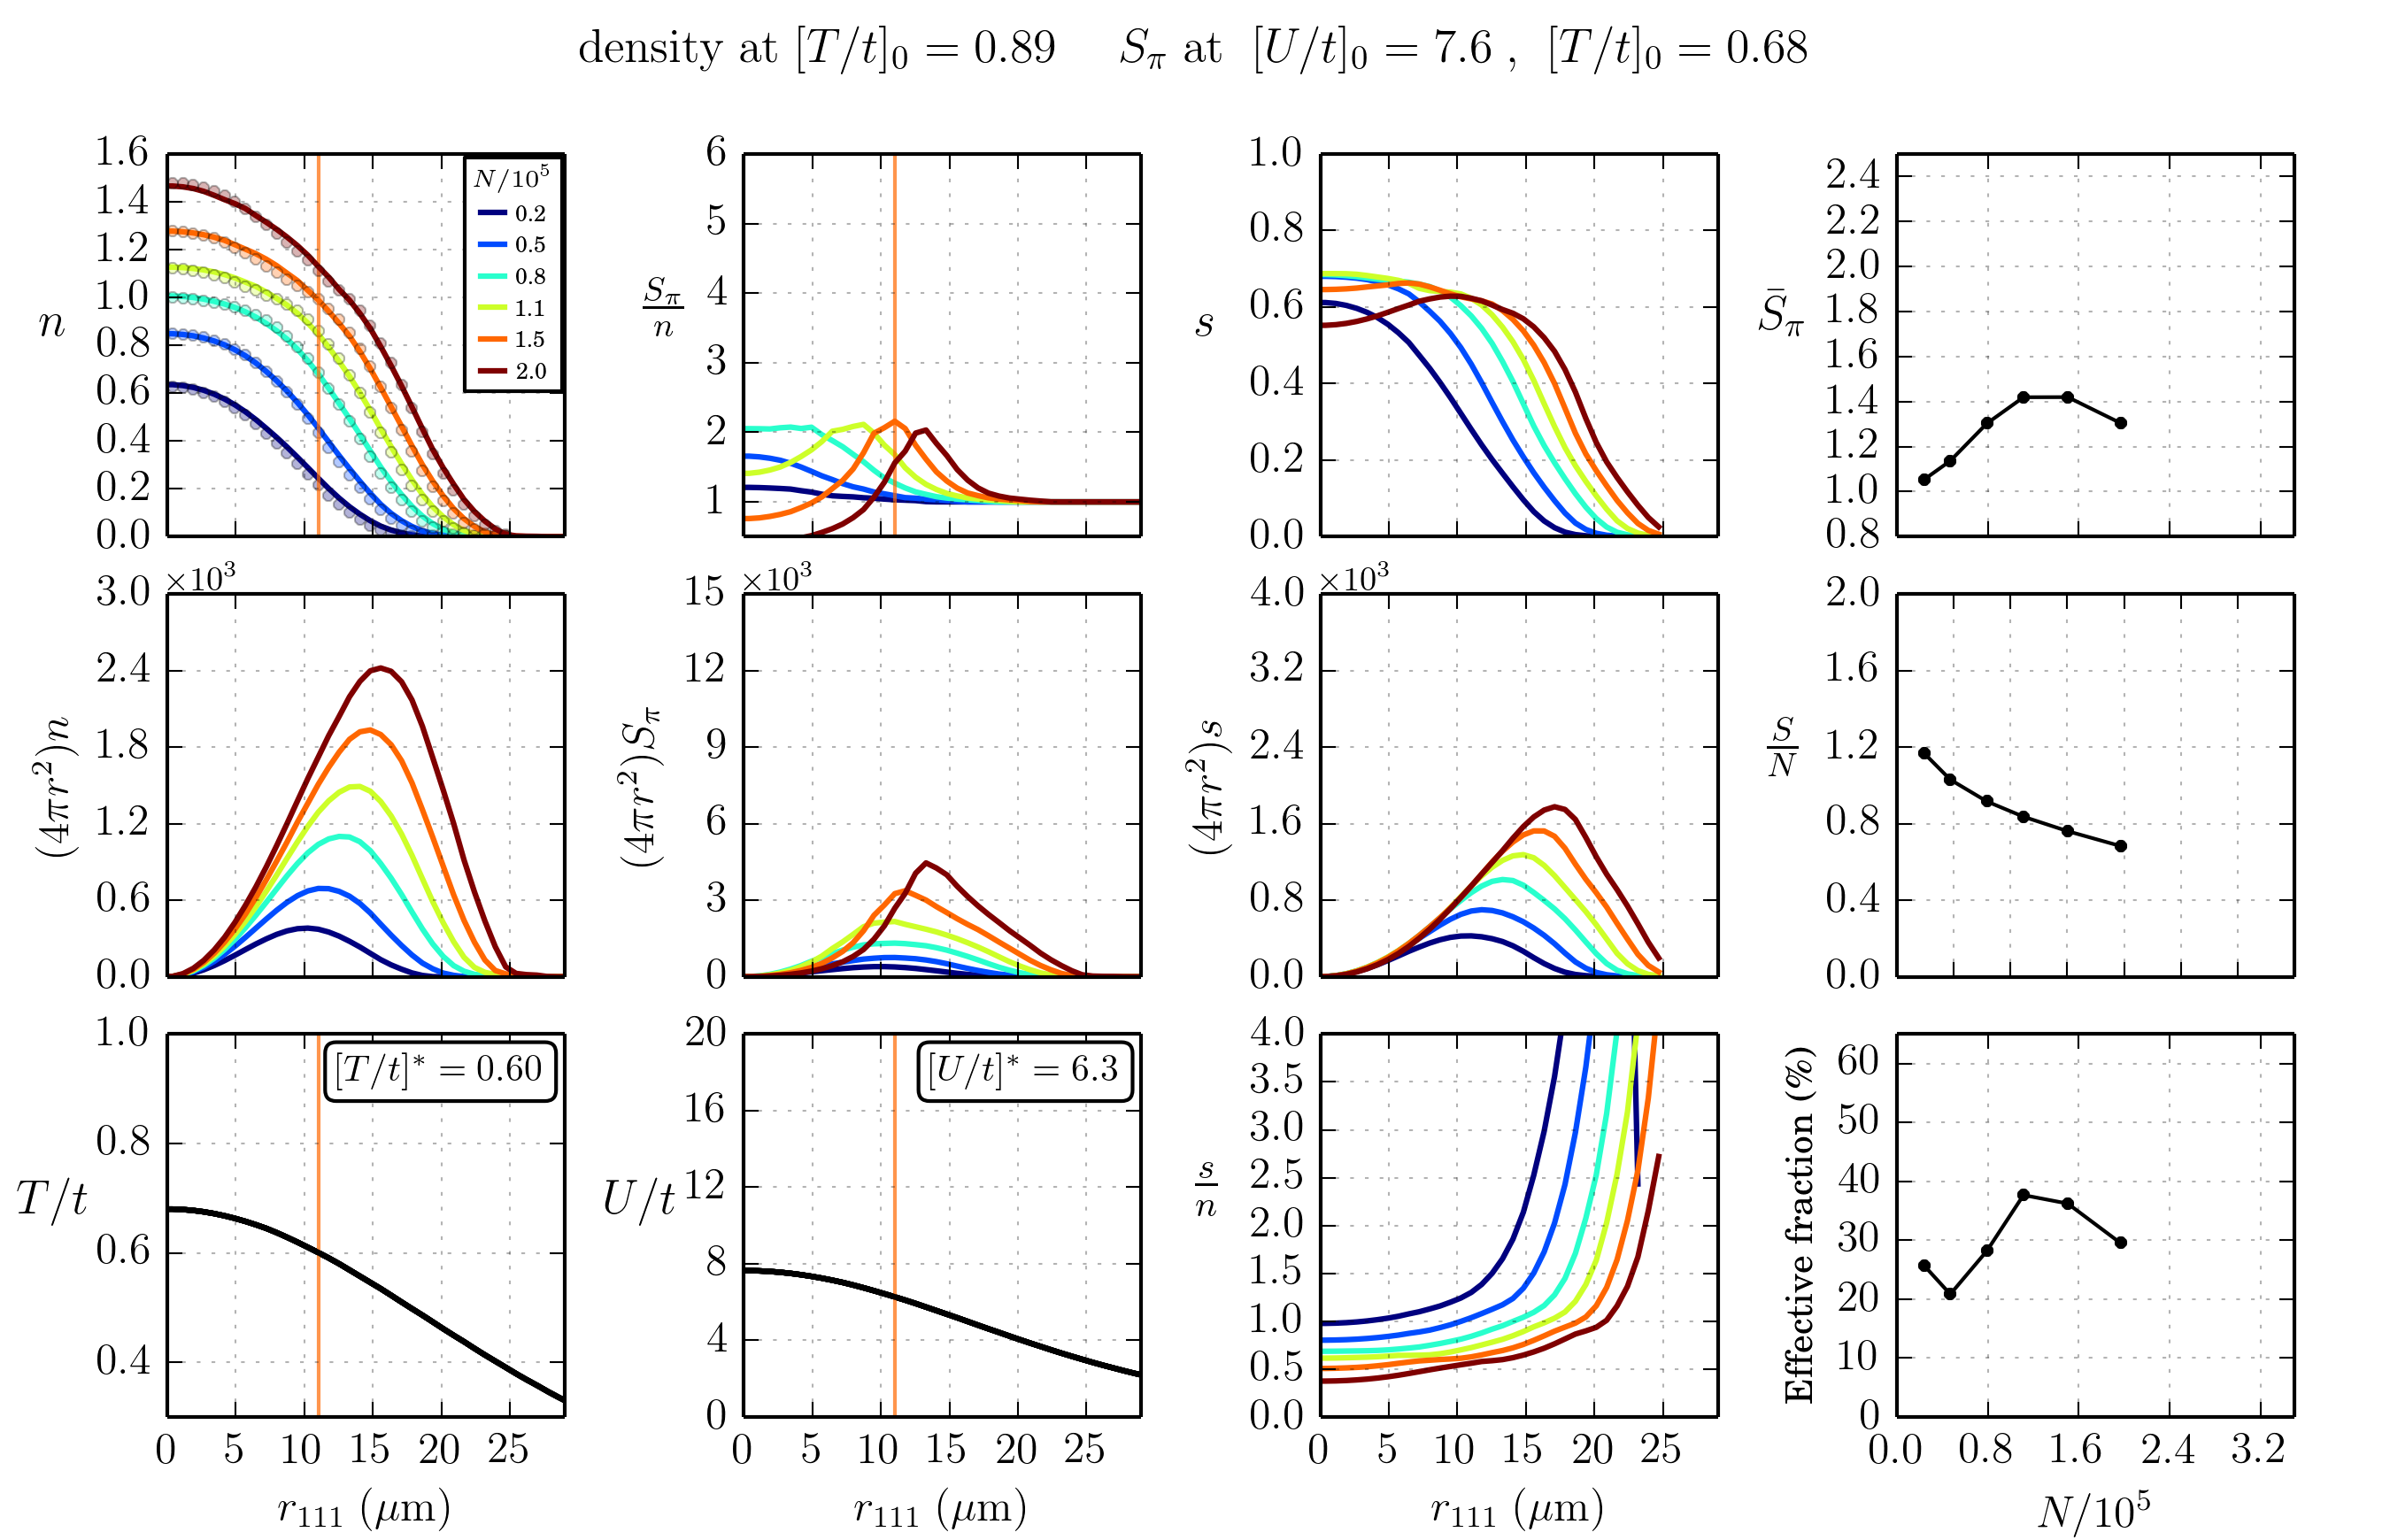
\includegraphics[width=0.95\textwidth]{figures/200a0_hot.png}
\caption{Scattering length 200\,$a_{0}$ ($[U/t]_{0}=7.6$).  } 
\label{fig:200a0_varyNhot}
\end{figure}
\begin{figure}[H]
    \centering
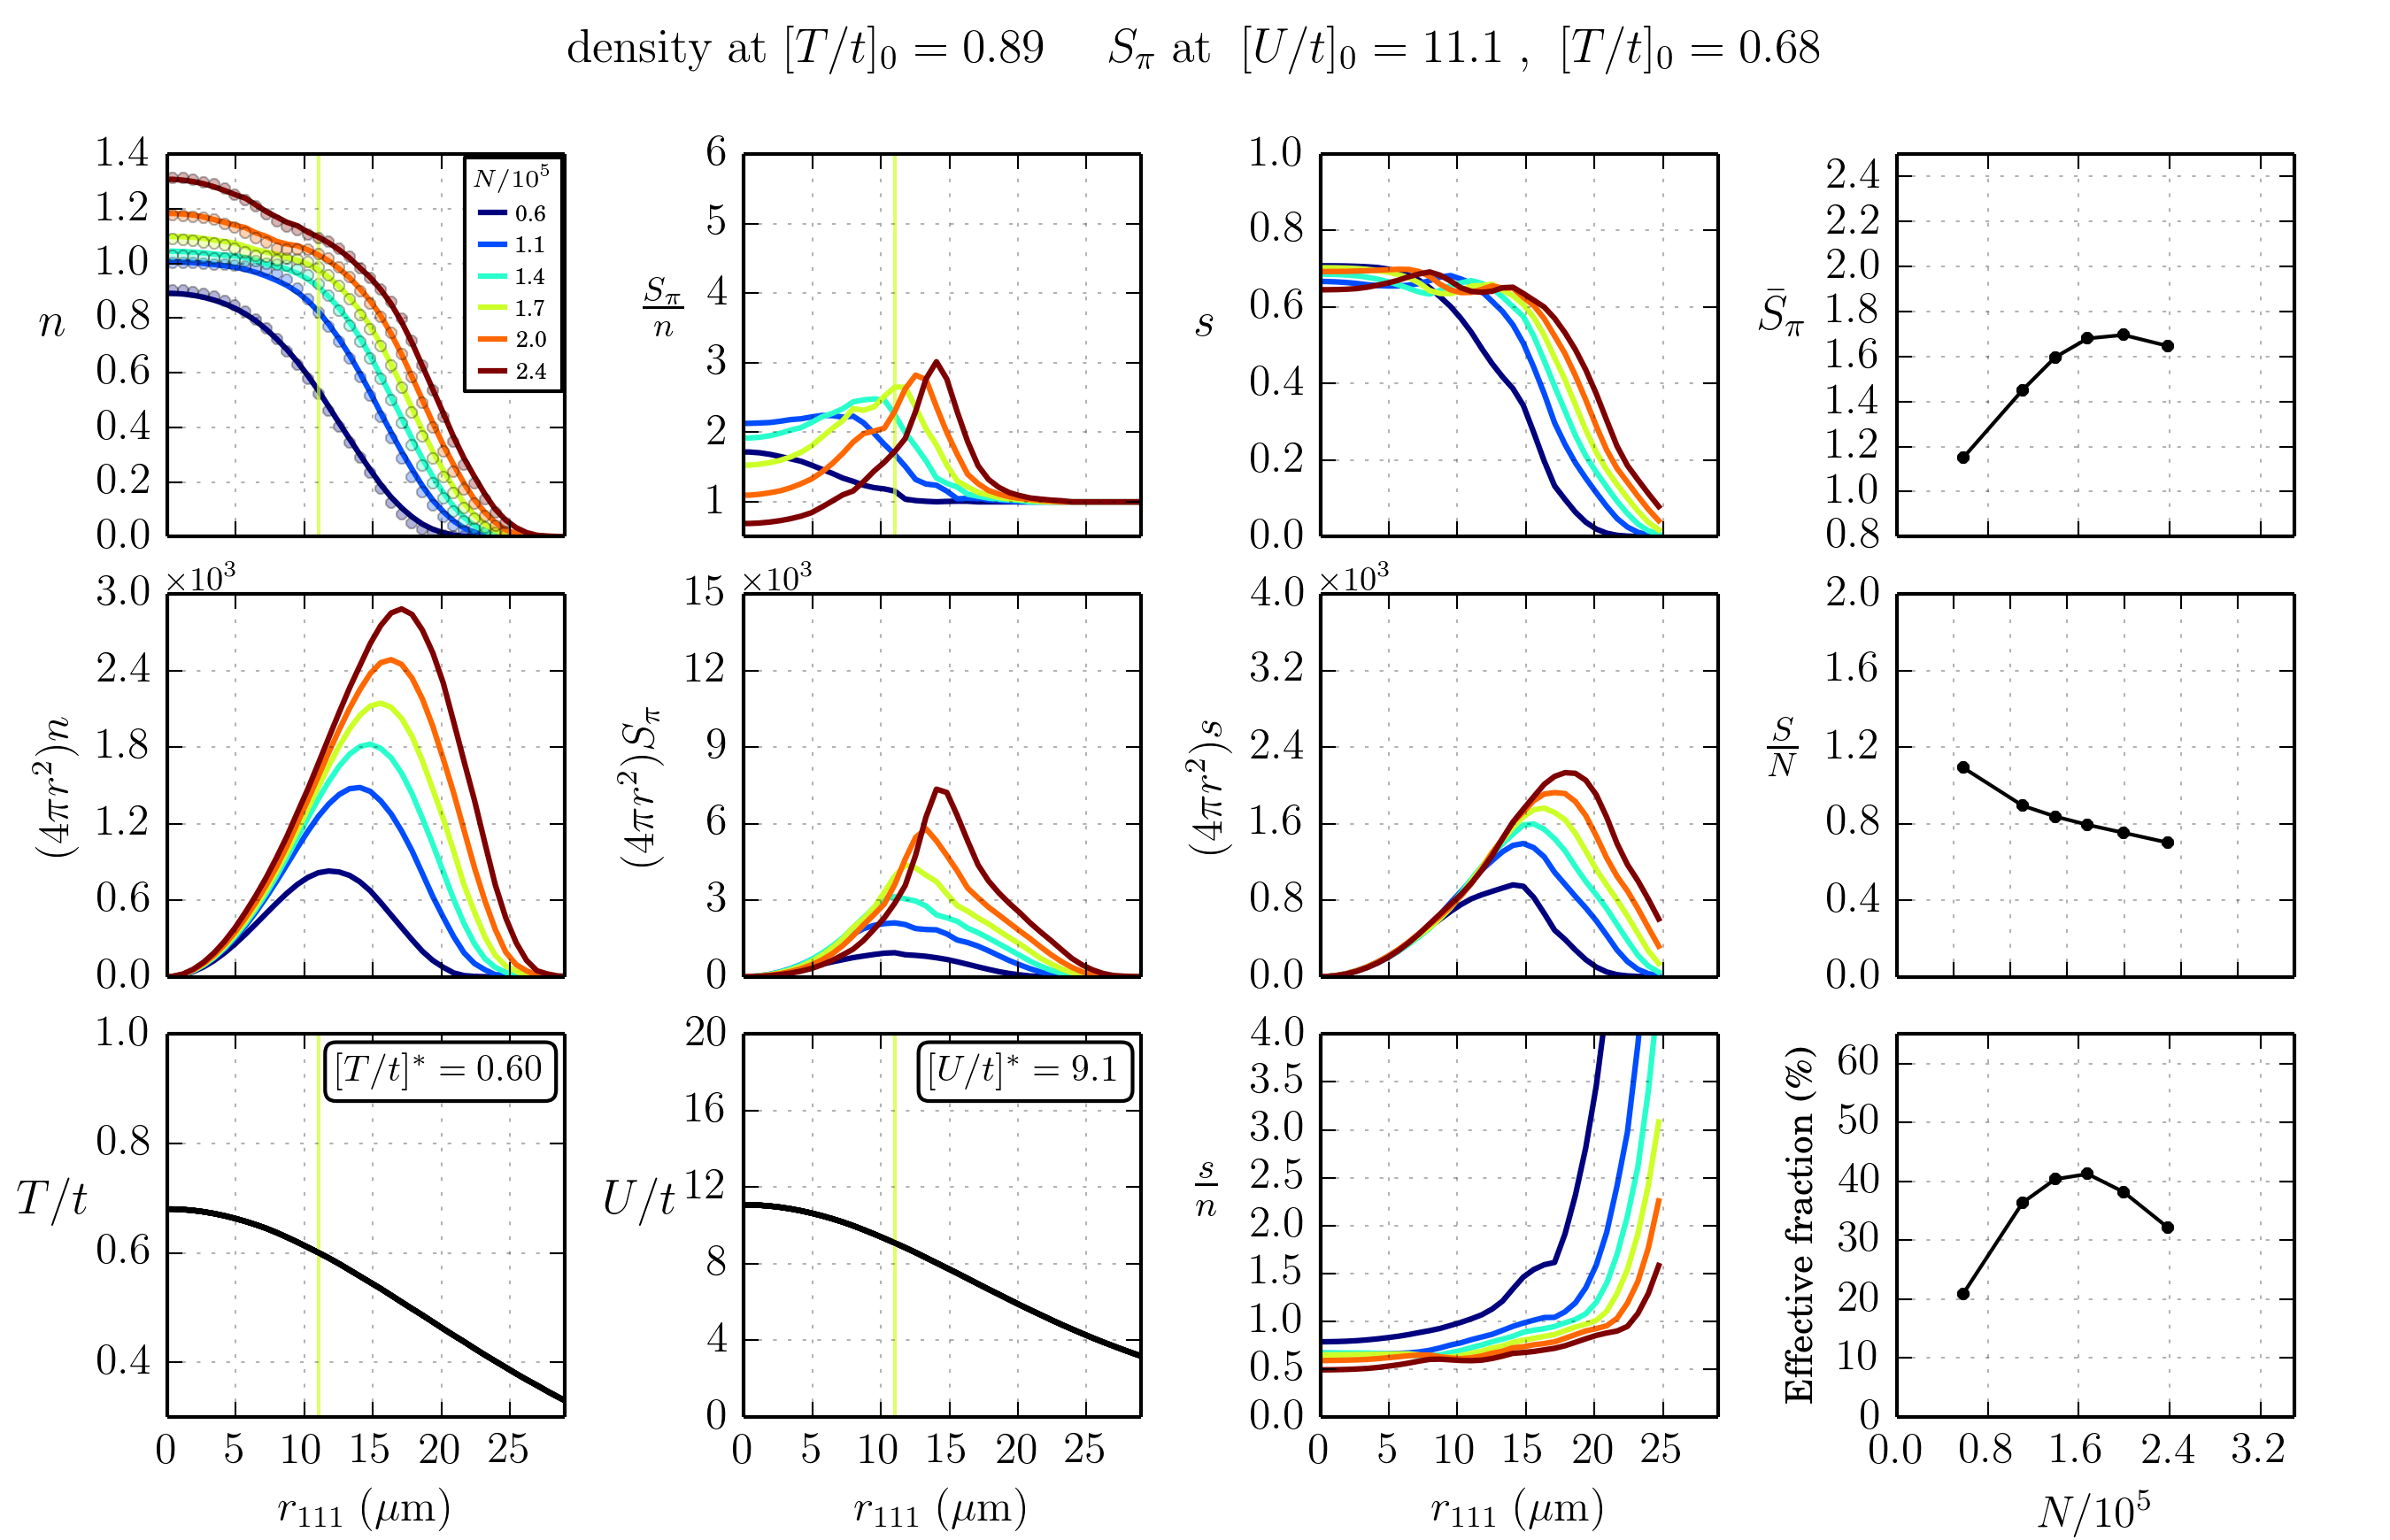
\includegraphics[width=0.95\textwidth]{figures/290a0_hot.png}
\caption{Scattering length 290\,$a_{0}$ ($[U/t]_{0}=11.1$).   } 
\label{fig:290a0_varyNhot}
\end{figure}
\begin{figure}[H]
    \centering
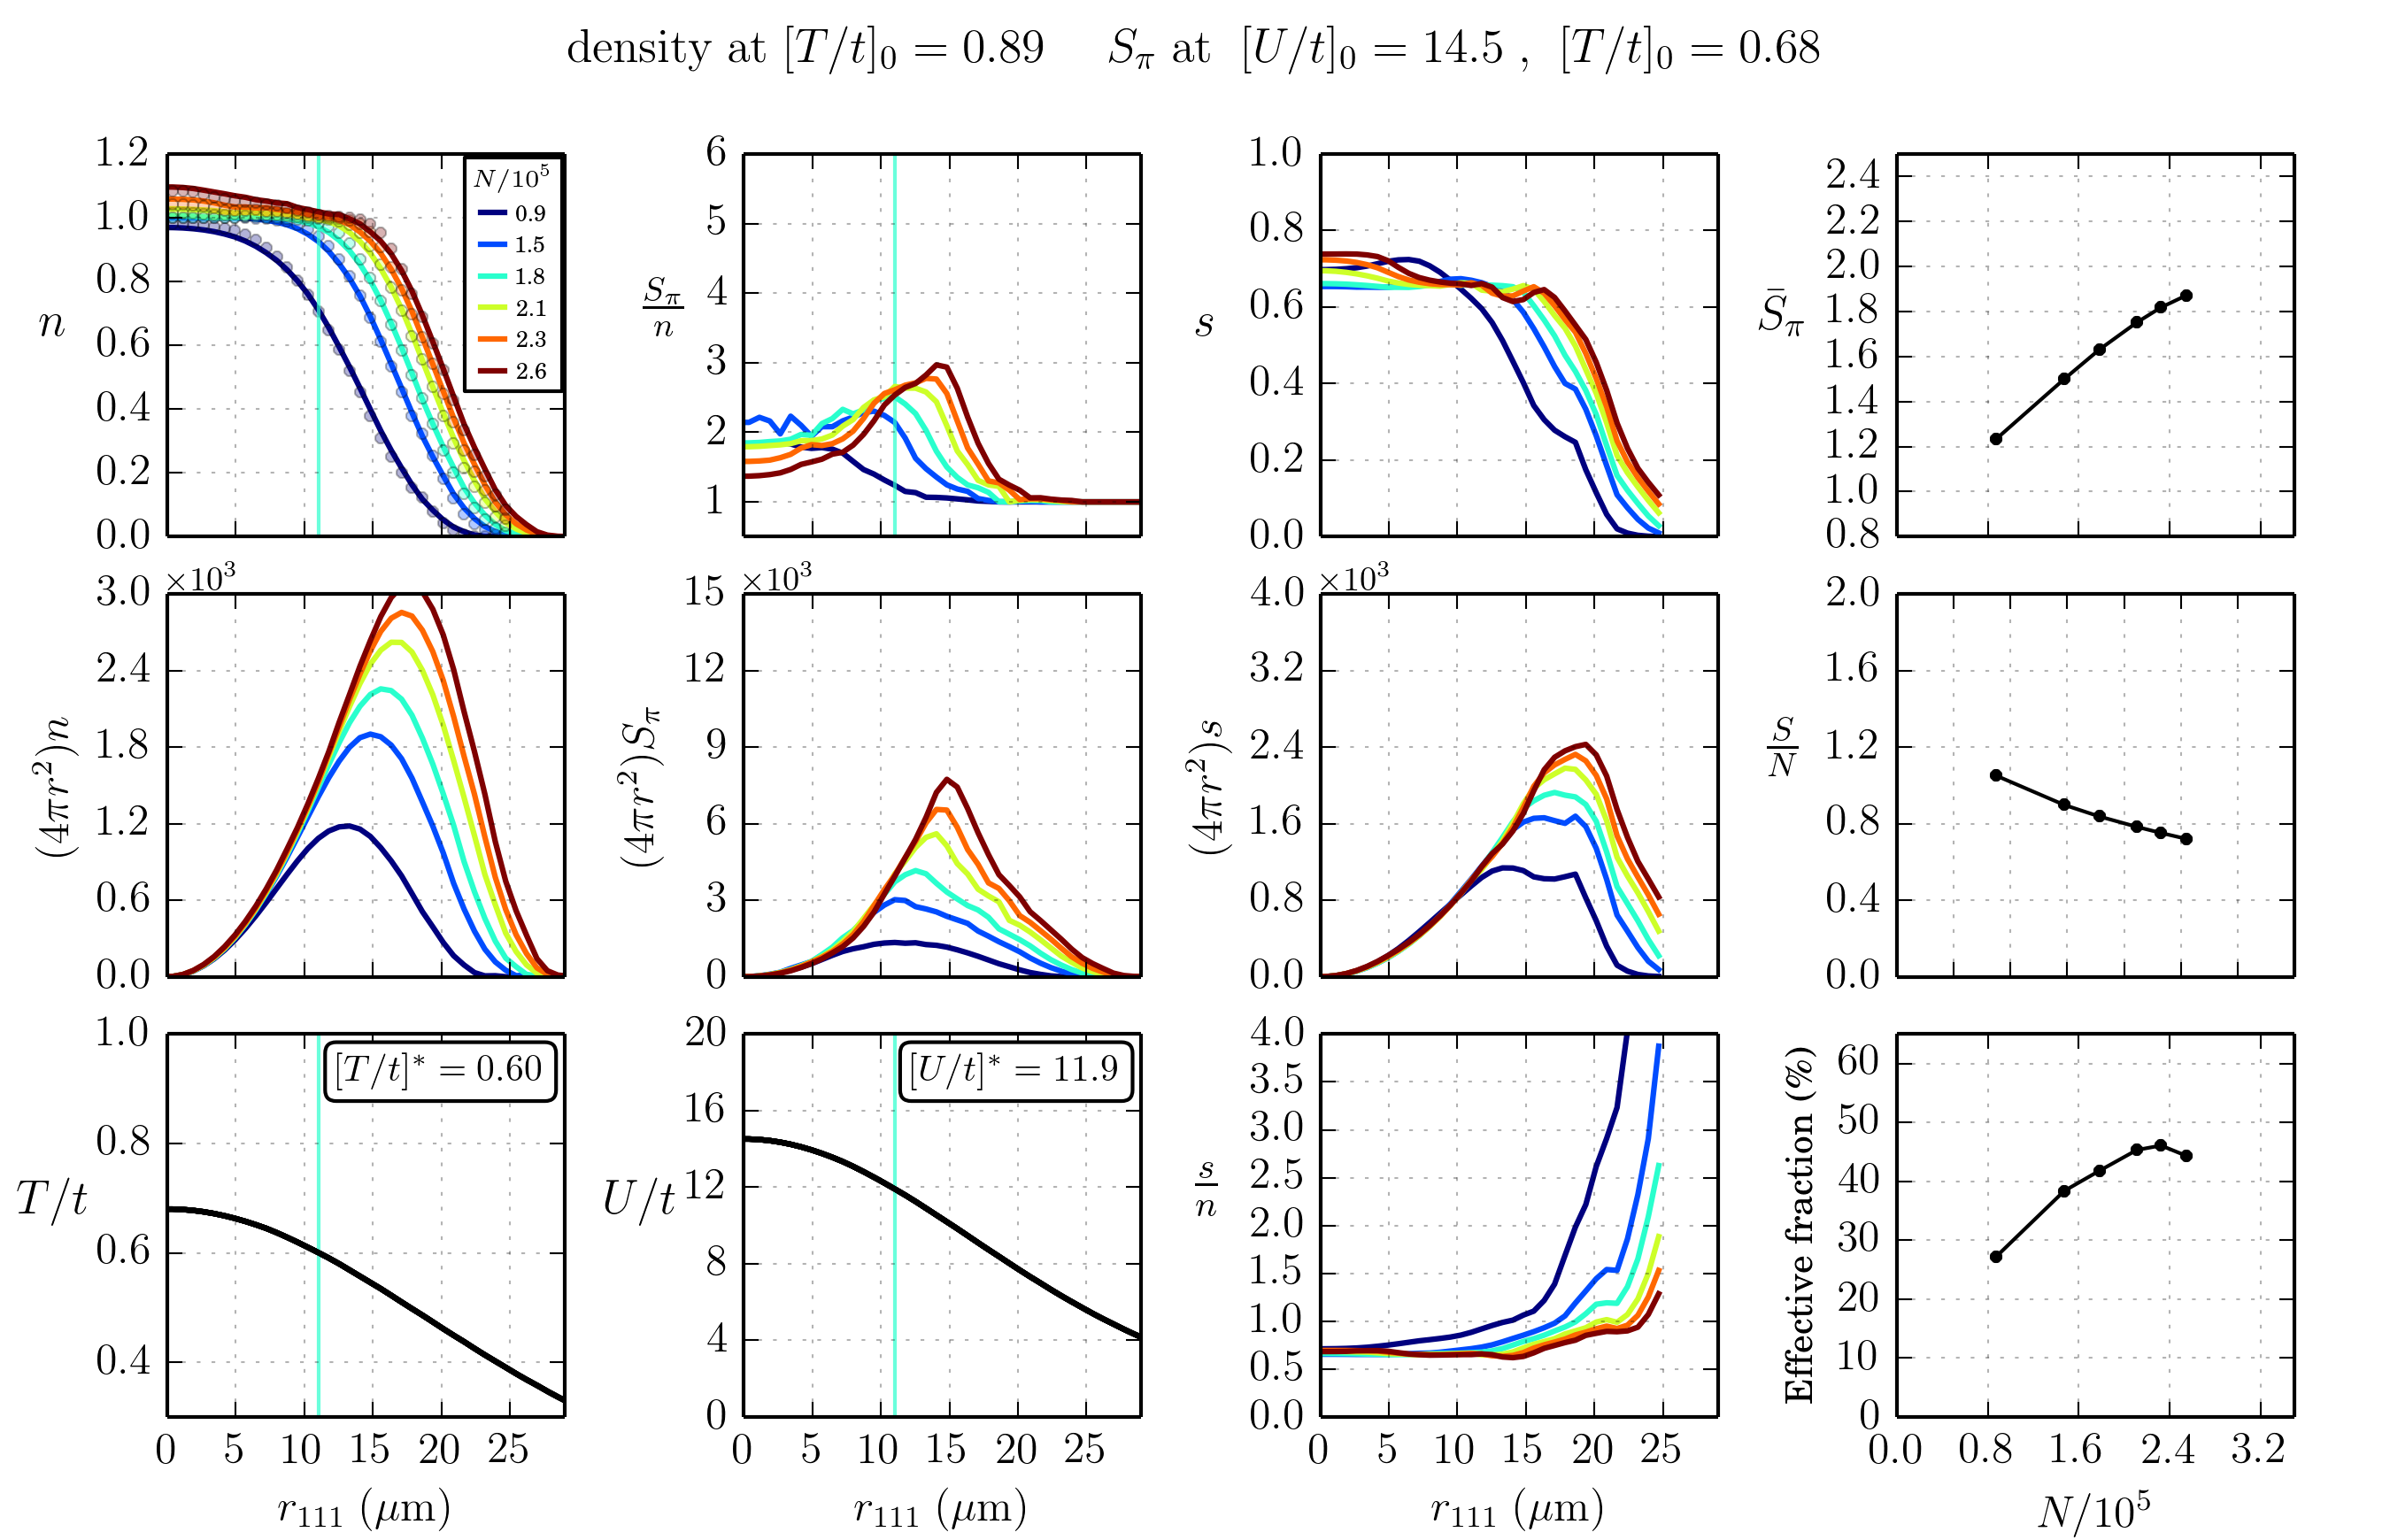
\includegraphics[width=0.95\textwidth]{figures/380a0_hot.png}
\caption{Scattering length 380\,$a_{0}$ ($[U/t]_{0}=14.5$).   } 
\label{fig:380a0_varyNhot}
\end{figure}
\begin{figure}[H]
    \centering
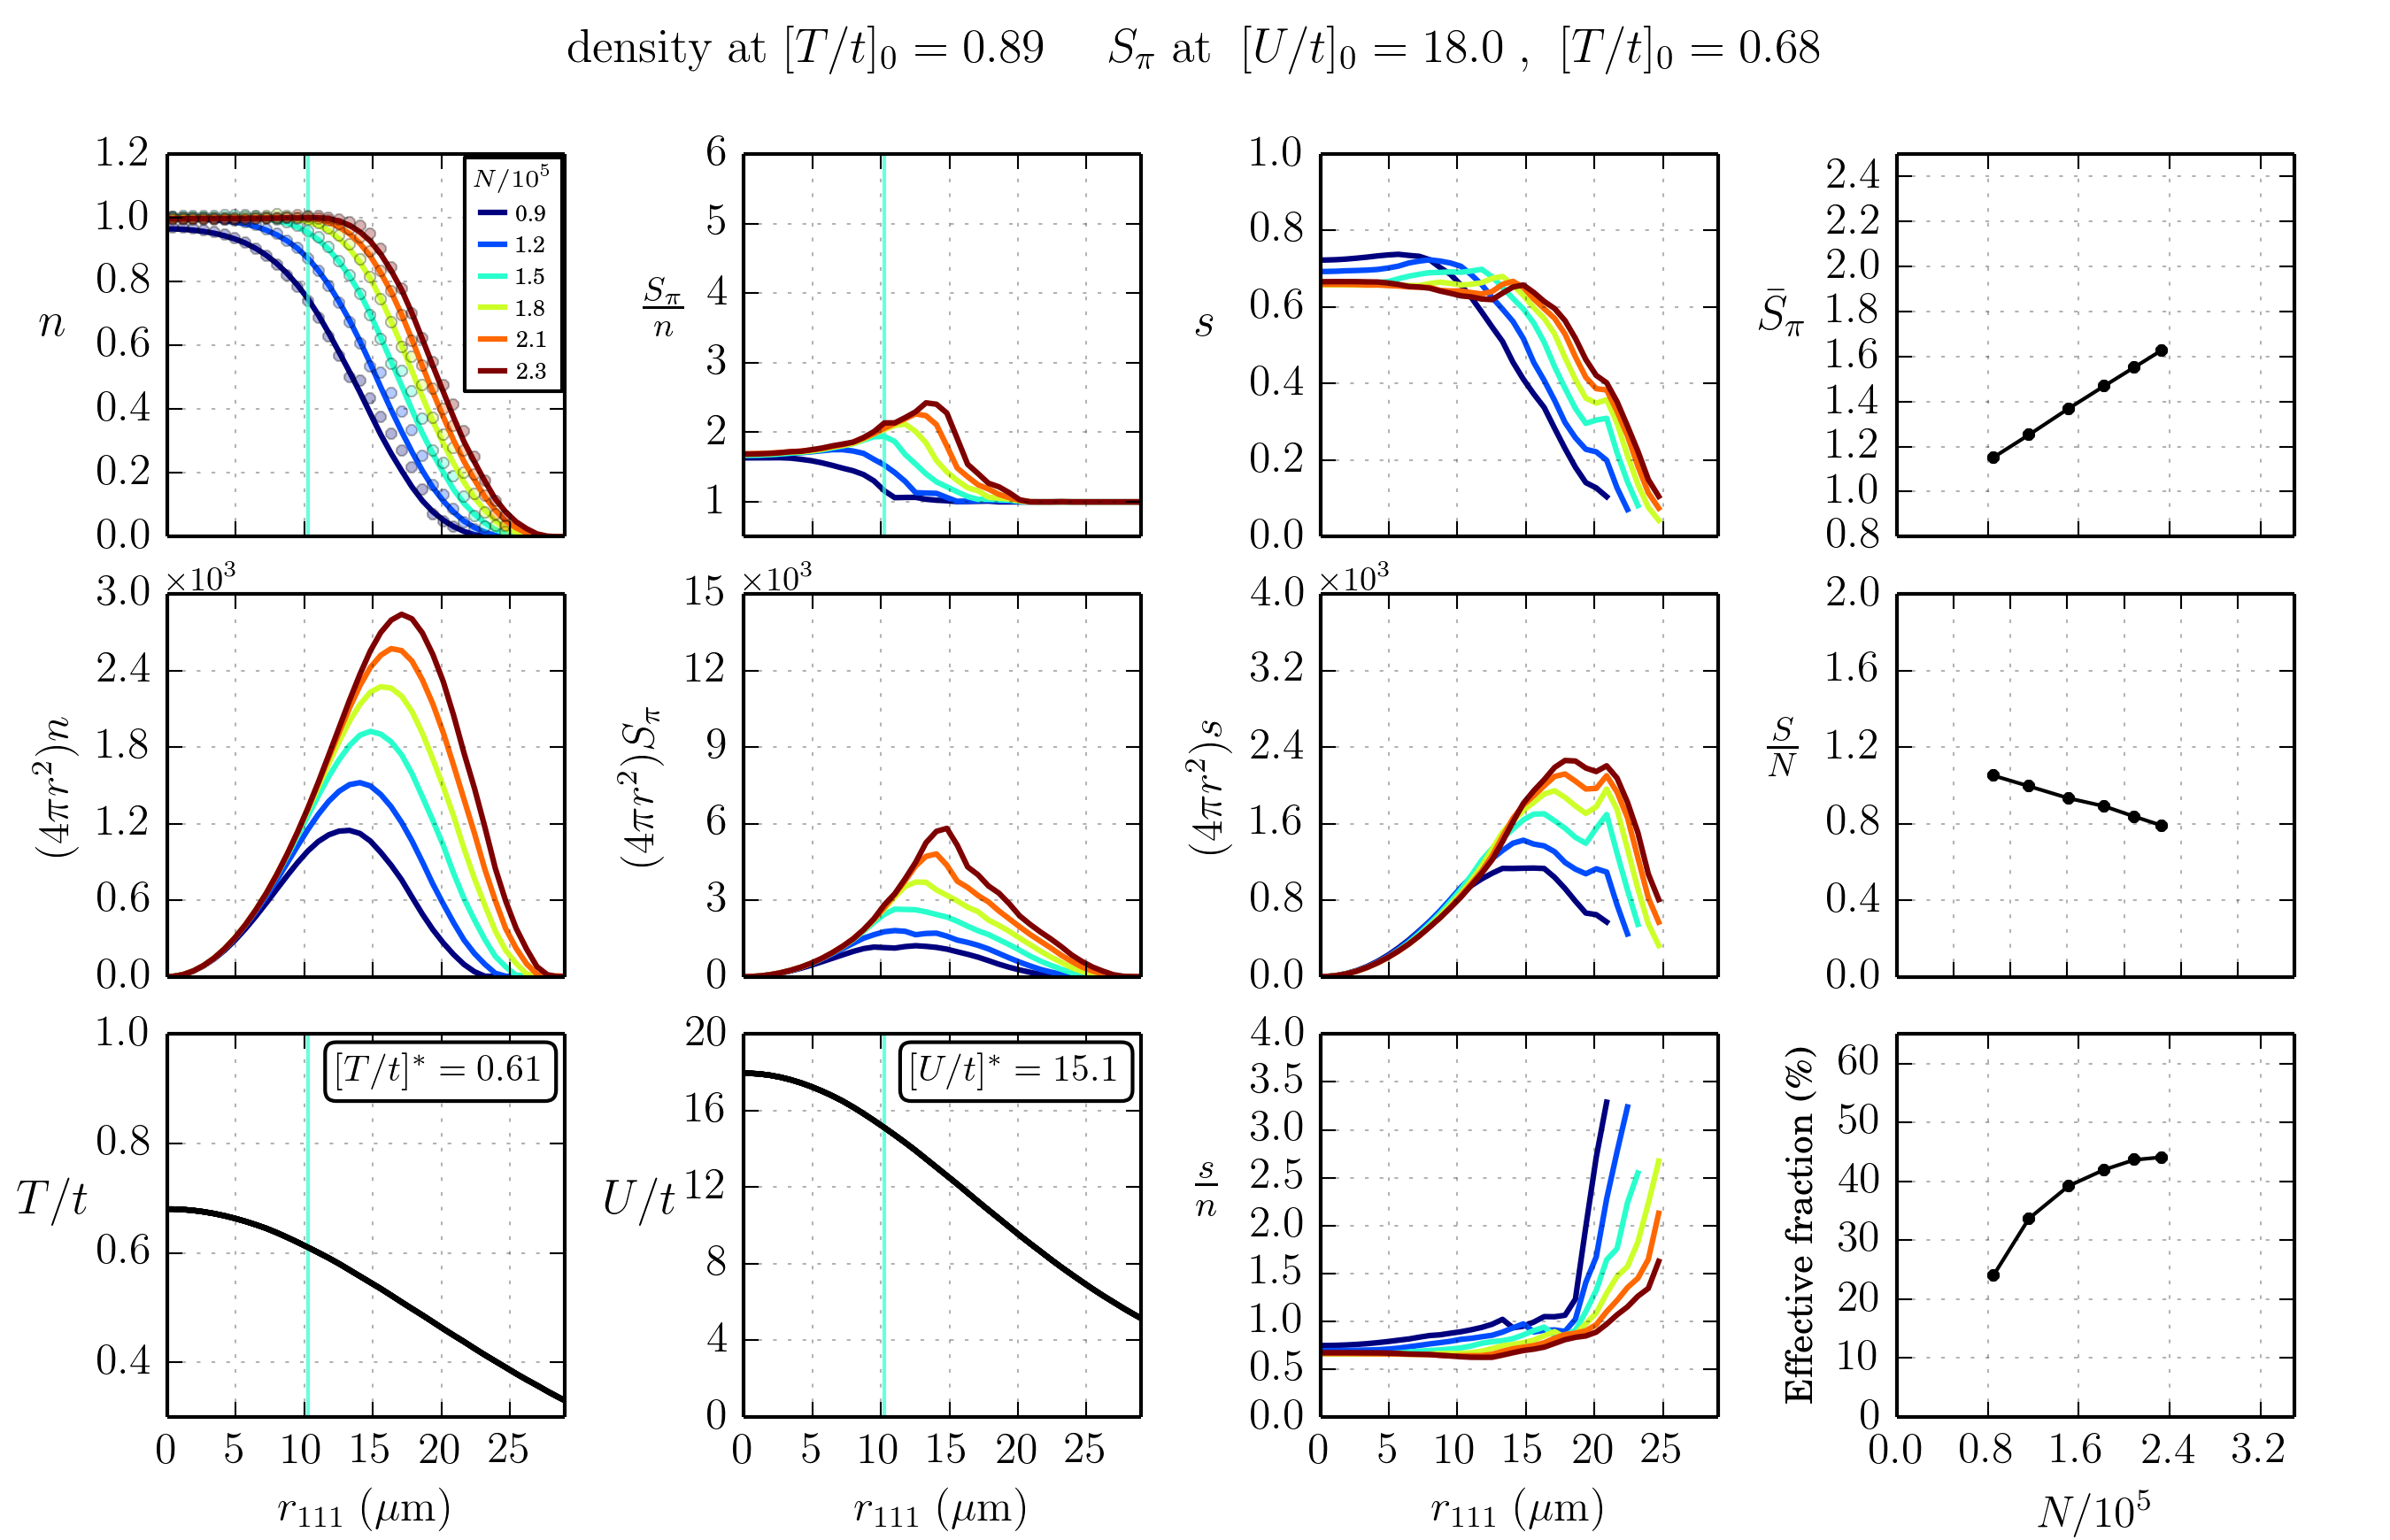
\includegraphics[width=0.95\textwidth]{figures/470a0_hot.png}
\caption{Scattering length 470\,$a_{0}$ ($[U/t]_{0}=18.0$).   } 
\label{fig:470a0_varyNhot}
\end{figure} 


\section{ LDA results for fixed atom number }  

Moving beyond the atom number variation,  we will focus on the LDA results
that match the atom number that peaks up Bragg in the experiment.  In this
case we vary only the temperature and observe the behavior of $\bar{S}_{\pi}$
with the goal of determining the temperature at which the LDA reproduces the
experimental data.   The results are shown in
Figs.~\ref{fig:200a0_varyT}-\ref{fig:470a0_varyT}.  

For all but the largest $[U/t]_{0}$ we were able to reach a low enough
temperature to cover the experimental data and its error bar.    Notice that
on the left panel the $x$-axis of the plot is given as $[T/t]_{0}$,  i.e.
the local value of $T/t$ at the center of our sample.   On the right panel
the $x$-axis is given as $[T/t]^{*}$,  the local value of $T/t$ at the radius
for which $S_{\pi}$ is maximized.   An equivalent notation is used for the
local value of $U/t$. 

Finally, if we can go ahead and find values of $T_{N}$ at the relevant
$[U/t]_{0}$  and $[U/t]^{*}$ we will be able to  quote these temperatures in
units of $T_{N}$.  

 
\begin{figure}
    \centering
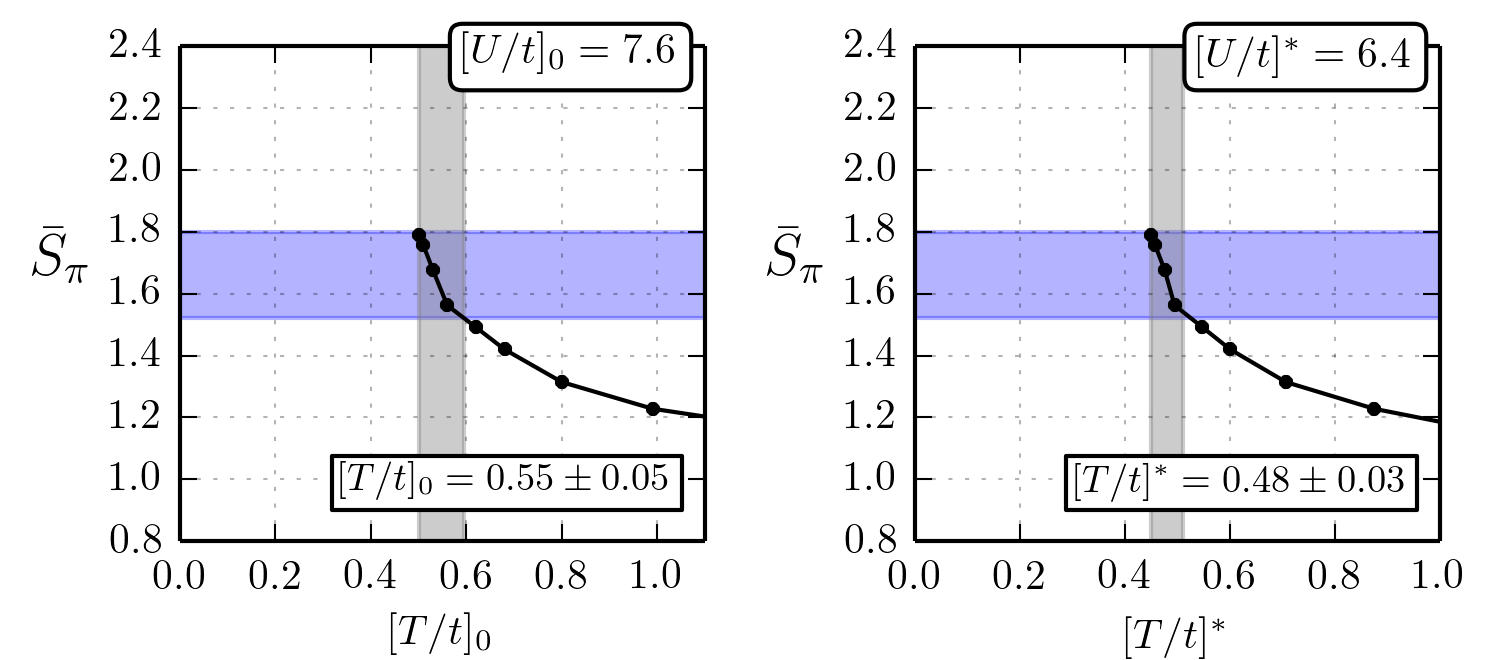
\includegraphics[width=0.95\textwidth]{figures/200a0_spi.png}
\caption{Scattering length 200\,$a_{0}$ ($[U/t]_{0}=7.6$).  } 
\label{fig:200a0_varyT}
\end{figure}
\begin{figure}
    \centering
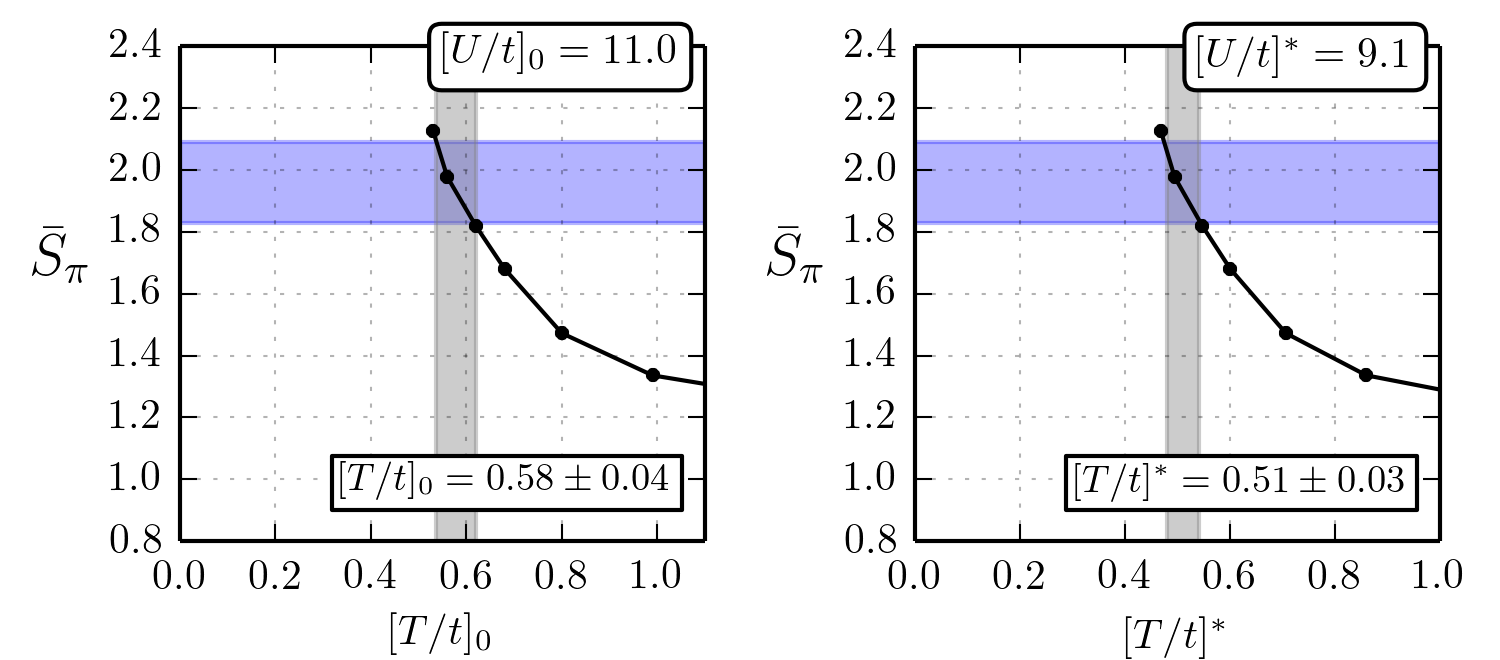
\includegraphics[width=0.95\textwidth]{figures/290a0_spi.png}
\caption{Scattering length 290\,$a_{0}$ ($[U/t]_{0}=11.1$).   } 
\label{fig:290a0_varyT}
\end{figure}
\begin{figure}
    \centering
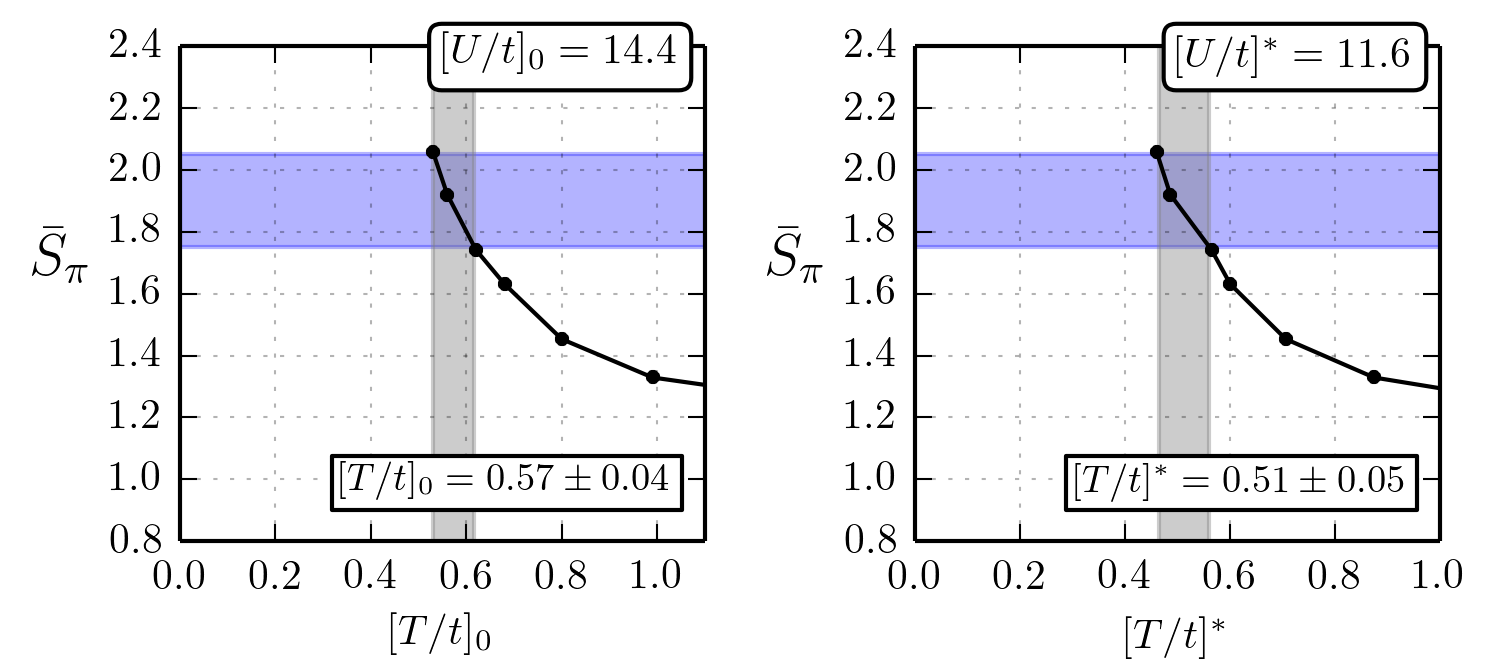
\includegraphics[width=0.95\textwidth]{figures/380a0_spi.png}
\caption{Scattering length 380\,$a_{0}$ ($[U/t]_{0}=14.5$).   } 
\label{fig:380a0_varyT}
\end{figure}
\begin{figure}
    \centering
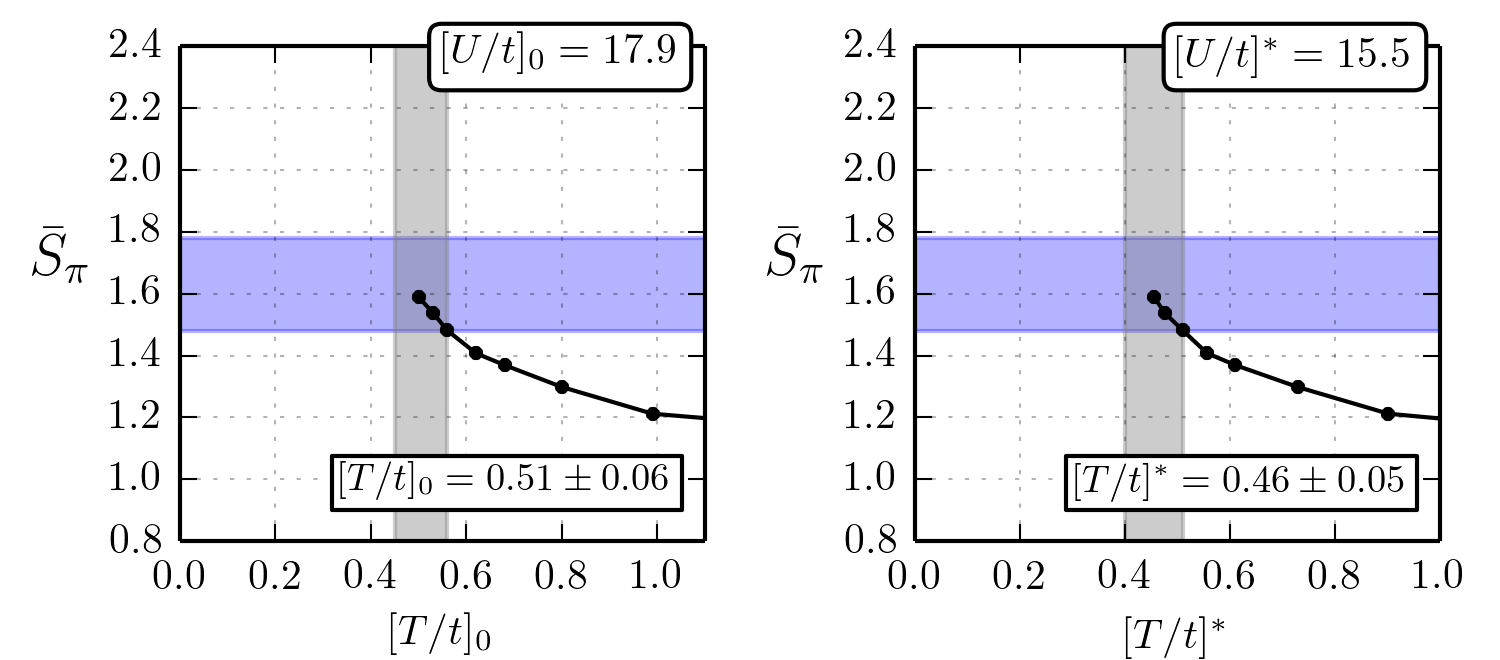
\includegraphics[width=0.95\textwidth]{figures/470a0_spi.png}
\caption{Scattering length 470\,$a_{0}$ ($[U/t]_{0}=18.0$).   } 
\label{fig:470a0_varyT}
\end{figure} 

 
 

 
\bibliographystyle{osa} \bibliography{latt_evap}

\end{document}




